% Created 2024-06-26 Wed 11:39
% Intended LaTeX compiler: xelatex
\documentclass[11pt]{article}
\usepackage{hyperref}
% wrong resolution of image
% https://tex.stackexchange.com/questions/21627/image-from-includegraphics-showing-in-wrong-image-size?rq=1

%%%%%%%%%%%%%%%%%%%%%%%%%%%%%%%%%%%%%%
%% TIPS                                 %%
%%%%%%%%%%%%%%%%%%%%%%%%%%%%%%%%%%%%%%
% \substack{a\\b} for multiple lines text
% \usepackage{expl3}
% \expandafter\def\csname ver@l3regex.sty\endcsname{}
% \usepackage{pkgloader}
\usepackage[utf8]{inputenc}

% nfss error
% \usepackage[B1,T1]{fontenc}
\usepackage{fontspec}

% \usepackage[Emoticons]{ucharclasses}
\newfontfamily\DejaSans{DejaVu Sans}
% \setDefaultTransitions{\DejaSans}{}

% pdfplots will load xolor automatically without option
\usepackage[dvipsnames]{xcolor}

%                                                             ┳┳┓   ┓
%                                                             ┃┃┃┏┓╋┣┓
%                                                             ┛ ┗┗┻┗┛┗
% \usepackage{amsmath} mathtools loads the amsmath
\usepackage{amsmath}
\usepackage{mathtools}

\usepackage{amsthm}
\usepackage{amsbsy}

%\usepackage{commath}

\usepackage{amssymb}

\usepackage{mathrsfs}
%\usepackage{mathabx}
\usepackage{stmaryrd}
\usepackage{empheq}

\usepackage{scalerel}
\usepackage{stackengine}
\usepackage{stackrel}



\usepackage{nicematrix}
\usepackage{tensor}
\usepackage{blkarray}
\usepackage{siunitx}
\usepackage[f]{esvect}

% centering \not on a letter
\usepackage{slashed}
\usepackage[makeroom]{cancel}

%\usepackage{merriweather}
\usepackage{unicode-math}
\setmainfont{TeX Gyre Pagella}
% \setmathfont{STIX}
%\setmathfont{texgyrepagella-math.otf}
%\setmathfont{Libertinus Math}
\setmathfont{Latin Modern Math}

 % \setmathfont[range={\smwhtdiamond,\enclosediamond,\varlrtriangle}]{Latin Modern Math}
\setmathfont[range={\rightrightarrows,\twoheadrightarrow,\leftrightsquigarrow,\triangledown,\vartriangle,\precneq,\succneq,\prec,\succ,\preceq,\succeq,\tieconcat}]{XITS Math}
 \setmathfont[range={\int,\setminus}]{Libertinus Math}
 % \setmathfont[range={\mathalpha}]{TeX Gyre Pagella Math}
%\setmathfont[range={\mitA,\mitB,\mitC,\mitD,\mitE,\mitF,\mitG,\mitH,\mitI,\mitJ,\mitK,\mitL,\mitM,\mitN,\mitO,\mitP,\mitQ,\mitR,\mitS,\mitT,\mitU,\mitV,\mitW,\mitX,\mitY,\mitZ,\mita,\mitb,\mitc,\mitd,\mite,\mitf,\mitg,\miti,\mitj,\mitk,\mitl,\mitm,\mitn,\mito,\mitp,\mitq,\mitr,\mits,\mitt,\mitu,\mitv,\mitw,\mitx,\mity,\mitz}]{TeX Gyre Pagella Math}
% unicode is not good at this!
%\let\nmodels\nvDash

 \usepackage{wasysym}

 % for wide hat
 \DeclareSymbolFont{yhlargesymbols}{OMX}{yhex}{m}{n} \DeclareMathAccent{\what}{\mathord}{yhlargesymbols}{"62}

%                                                               ┏┳┓•┓
%                                                                ┃ ┓┃┏┓
%                                                                ┻ ┗┛┗┗

\usepackage{pgfplots}
\pgfplotsset{compat=1.18}
\usepackage{tikz}
\usepackage{tikz-cd}
\tikzcdset{scale cd/.style={every label/.append style={scale=#1},
    cells={nodes={scale=#1}}}}
% TODO: discard qtree and use forest
% \usepackage{tikz-qtree}
\usepackage{forest}

\usetikzlibrary{arrows,positioning,calc,fadings,decorations,matrix,decorations,shapes.misc}
%setting from geogebra
\definecolor{ccqqqq}{rgb}{0.8,0,0}

%                                                          ┳┳┓•    ┓┓
%                                                          ┃┃┃┓┏┏┏┓┃┃┏┓┏┓┏┓┏┓┓┏┏
%                                                          ┛ ┗┗┛┗┗ ┗┗┗┻┛┗┗ ┗┛┗┻┛
%\usepackage{twemojis}
\usepackage[most]{tcolorbox}
\usepackage{threeparttable}
\usepackage{tabularx}

\usepackage{enumitem}
\usepackage[indLines=false]{algpseudocodex}
\usepackage[]{algorithm2e}
% \SetKwComment{Comment}{/* }{ */}
% \algrenewcommand\algorithmicrequire{\textbf{Input:}}
% \algrenewcommand\algorithmicensure{\textbf{Output:}}
% wrong with preview
\usepackage{subcaption}
\usepackage{caption}
% {\aunclfamily\Huge}
\usepackage{auncial}

\usepackage{float}

\usepackage{fancyhdr}

\usepackage{ifthen}
\usepackage{xargs}

\definecolor{mintedbg}{rgb}{0.99,0.99,0.99}
\usepackage[cachedir=\detokenize{~/miscellaneous/trash}]{minted}
\setminted{breaklines,
  mathescape,
  bgcolor=mintedbg,
  fontsize=\footnotesize,
  frame=single,
  linenos}
\usemintedstyle{xcode}
\usepackage{tcolorbox}
\usepackage{etoolbox}



\usepackage{imakeidx}
\usepackage{hyperref}
\usepackage{soul}
\usepackage{framed}

% don't use this for preview
%\usepackage[margin=1.5in]{geometry}
% \usepackage{geometry}
% \geometry{legalpaper, landscape, margin=1in}
\usepackage[font=itshape]{quoting}

%\LoadPackagesNow
%\usepackage[xetex]{preview}
%%%%%%%%%%%%%%%%%%%%%%%%%%%%%%%%%%%%%%%
%% USEPACKAGES end                       %%
%%%%%%%%%%%%%%%%%%%%%%%%%%%%%%%%%%%%%%%

%%%%%%%%%%%%%%%%%%%%%%%%%%%%%%%%%%%%%%%
%% Algorithm environment
%%%%%%%%%%%%%%%%%%%%%%%%%%%%%%%%%%%%%%%
\SetKwIF{Recv}{}{}{upon receiving}{do}{}{}{}
\SetKwBlock{Init}{initially do}{}
\SetKwProg{Function}{Function}{:}{}

% https://github.com/chrmatt/algpseudocodex/issues/3
\algnewcommand\algorithmicswitch{\textbf{switch}}%
\algnewcommand\algorithmiccase{\textbf{case}}
\algnewcommand\algorithmicof{\textbf{of}}
\algnewcommand\algorithmicotherwise{\texttt{otherwise} $\Rightarrow$}

\makeatletter
\algdef{SE}[SWITCH]{Switch}{EndSwitch}[1]{\algpx@startIndent\algpx@startCodeCommand\algorithmicswitch\ #1\ \algorithmicdo}{\algpx@endIndent\algpx@startCodeCommand\algorithmicend\ \algorithmicswitch}%
\algdef{SE}[CASE]{Case}{EndCase}[1]{\algpx@startIndent\algpx@startCodeCommand\algorithmiccase\ #1}{\algpx@endIndent\algpx@startCodeCommand\algorithmicend\ \algorithmiccase}%
\algdef{SE}[CASEOF]{CaseOf}{EndCaseOf}[1]{\algpx@startIndent\algpx@startCodeCommand\algorithmiccase\ #1 \algorithmicof}{\algpx@endIndent\algpx@startCodeCommand\algorithmicend\ \algorithmiccase}
\algdef{SE}[OTHERWISE]{Otherwise}{EndOtherwise}[0]{\algpx@startIndent\algpx@startCodeCommand\algorithmicotherwise}{\algpx@endIndent\algpx@startCodeCommand\algorithmicend\ \algorithmicotherwise}
\ifbool{algpx@noEnd}{%
  \algtext*{EndSwitch}%
  \algtext*{EndCase}%
  \algtext*{EndCaseOf}
  \algtext*{EndOtherwise}
  %
  % end indent line after (not before), to get correct y position for multiline text in last command
  \apptocmd{\EndSwitch}{\algpx@endIndent}{}{}%
  \apptocmd{\EndCase}{\algpx@endIndent}{}{}%
  \apptocmd{\EndCaseOf}{\algpx@endIndent}{}{}
  \apptocmd{\EndOtherwise}{\algpx@endIndent}{}{}
}{}%

\pretocmd{\Switch}{\algpx@endCodeCommand}{}{}
\pretocmd{\Case}{\algpx@endCodeCommand}{}{}
\pretocmd{\CaseOf}{\algpx@endCodeCommand}{}{}
\pretocmd{\Otherwise}{\algpx@endCodeCommand}{}{}

% for end commands that may not be printed, tell endCodeCommand whether we are using noEnd
\ifbool{algpx@noEnd}{%
  \pretocmd{\EndSwitch}{\algpx@endCodeCommand[1]}{}{}%
  \pretocmd{\EndCase}{\algpx@endCodeCommand[1]}{}{}
  \pretocmd{\EndCaseOf}{\algpx@endCodeCommand[1]}{}{}%
  \pretocmd{\EndOtherwise}{\algpx@endCodeCommand[1]}{}{}
}{%
  \pretocmd{\EndSwitch}{\algpx@endCodeCommand[0]}{}{}%
  \pretocmd{\EndCase}{\algpx@endCodeCommand[0]}{}{}%
  \pretocmd{\EndCaseOf}{\algpx@endCodeCommand[0]}{}{}
  \pretocmd{\EndOtherwise}{\algpx@endCodeCommand[0]}{}{}
}%
\makeatother
% % For algpseudocode
% \algnewcommand\algorithmicswitch{\textbf{switch}}
% \algnewcommand\algorithmiccase{\textbf{case}}
% \algnewcommand\algorithmiccaseof{\textbf{case}}
% \algnewcommand\algorithmicof{\textbf{of}}
% % New "environments"
% \algdef{SE}[SWITCH]{Switch}{EndSwitch}[1]{\algorithmicswitch\ #1\ \algorithmicdo}{\algorithmicend\ \algorithmicswitch}%
% \algdef{SE}[CASE]{Case}{EndCase}[1]{\algorithmiccase\ #1}{\algorithmicend\ \algorithmiccase}%
% \algtext*{EndSwitch}%
% \algtext*{EndCase}
% \algdef{SE}[CASEOF]{CaseOf}{EndCaseOf}[1]{\algorithmiccaseof\ #1 \algorithmicof}{\algorithmicend\ \algorithmiccaseof}
% \algtext*{EndCaseOf}



%\pdfcompresslevel0

% quoting from
% https://tex.stackexchange.com/questions/391726/the-quotation-environment
\NewDocumentCommand{\bywhom}{m}{% the Bourbaki trick
  {\nobreak\hfill\penalty50\hskip1em\null\nobreak
   \hfill\mbox{\normalfont(#1)}%
   \parfillskip=0pt \finalhyphendemerits=0 \par}%
}

\NewDocumentEnvironment{pquotation}{m}
  {\begin{quoting}[
     indentfirst=true,
     leftmargin=\parindent,
     rightmargin=\parindent]\itshape}
  {\bywhom{#1}\end{quoting}}

\indexsetup{othercode=\small}
\makeindex[columns=2,options={-s /media/wu/file/stuuudy/notes/index_style.ist},intoc]
\makeatletter
\def\@idxitem{\par\hangindent 0pt}
\makeatother


% \newcounter{dummy} \numberwithin{dummy}{section}
\newtheorem{dummy}{dummy}[section]
\theoremstyle{definition}
\newtheorem{definition}[dummy]{Definition}
\theoremstyle{plain}
\newtheorem{corollary}[dummy]{Corollary}
\newtheorem{lemma}[dummy]{Lemma}
\newtheorem{proposition}[dummy]{Proposition}
\newtheorem{theorem}[dummy]{Theorem}
\newtheorem{notation}[dummy]{Notation}
\newtheorem{conjecture}[dummy]{Conjecture}
\newtheorem{fact}[dummy]{Fact}
\newtheorem{warning}[dummy]{Warning}
\theoremstyle{definition}
\newtheorem{examplle}{Example}[section]
\theoremstyle{remark}
\newtheorem*{remark}{Remark}
\newtheorem{exercise}{Exercise}[subsection]
\newtheorem{problem}{Problem}[subsection]
\newtheorem{observation}{Observation}[section]
\newenvironment{claim}[1]{\par\noindent\textbf{Claim:}\space#1}{}

\makeatletter
\DeclareFontFamily{U}{tipa}{}
\DeclareFontShape{U}{tipa}{m}{n}{<->tipa10}{}
\newcommand{\arc@char}{{\usefont{U}{tipa}{m}{n}\symbol{62}}}%

\newcommand{\arc}[1]{\mathpalette\arc@arc{#1}}

\newcommand{\arc@arc}[2]{%
  \sbox0{$\m@th#1#2$}%
  \vbox{
    \hbox{\resizebox{\wd0}{\height}{\arc@char}}
    \nointerlineskip
    \box0
  }%
}
\makeatother

\setcounter{MaxMatrixCols}{20}
%%%%%%% ABS
\DeclarePairedDelimiter\abss{\lvert}{\rvert}%
\DeclarePairedDelimiter\normm{\lVert}{\rVert}%

% Swap the definition of \abs* and \norm*, so that \abs
% and \norm resizes the size of the brackets, and the
% starred version does not.
\makeatletter
\let\oldabs\abss
%\def\abs{\@ifstar{\oldabs}{\oldabs*}}
\newcommand{\abs}{\@ifstar{\oldabs}{\oldabs*}}
\newcommand{\norm}[1]{\left\lVert#1\right\rVert}
%\let\oldnorm\normm
%\def\norm{\@ifstar{\oldnorm}{\oldnorm*}}
%\renewcommand{norm}{\@ifstar{\oldnorm}{\oldnorm*}}
\makeatother

% \stackMath
% \newcommand\what[1]{%
% \savestack{\tmpbox}{\stretchto{%
%   \scaleto{%
%     \scalerel*[\widthof{\ensuremath{#1}}]{\kern-.6pt\bigwedge\kern-.6pt}%
%     {\rule[-\textheight/2]{1ex}{\textheight}}%WIDTH-LIMITED BIG WEDGE
%   }{\textheight}%
% }{0.5ex}}%
% \stackon[1pt]{#1}{\tmpbox}%
% }

% \newcommand\what[1]{\ThisStyle{%
%     \setbox0=\hbox{$\SavedStyle#1$}%
%     \stackengine{-1.0\ht0+.5pt}{$\SavedStyle#1$}{%
%       \stretchto{\scaleto{\SavedStyle\mkern.15mu\char'136}{2.6\wd0}}{1.4\ht0}%
%     }{O}{c}{F}{T}{S}%
%   }
% }

% \newcommand\wtilde[1]{\ThisStyle{%
%     \setbox0=\hbox{$\SavedStyle#1$}%
%     \stackengine{-.1\LMpt}{$\SavedStyle#1$}{%
%       \stretchto{\scaleto{\SavedStyle\mkern.2mu\AC}{.5150\wd0}}{.6\ht0}%
%     }{O}{c}{F}{T}{S}%
%   }
% }

% \newcommand\wbar[1]{\ThisStyle{%
%     \setbox0=\hbox{$\SavedStyle#1$}%
%     \stackengine{.5pt+\LMpt}{$\SavedStyle#1$}{%
%       \rule{\wd0}{\dimexpr.3\LMpt+.3pt}%
%     }{O}{c}{F}{T}{S}%
%   }
% }

\newcommand{\bl}[1] {\boldsymbol{#1}}
\newcommand{\Wt}[1] {\stackrel{\sim}{\smash{#1}\rule{0pt}{1.1ex}}}
\newcommand{\wt}[1] {\widetilde{#1}}
\newcommand{\tf}[1] {\textbf{#1}}

\newcommand{\wu}[1]{{\color{red} #1}}

%For boxed texts in align, use Aboxed{}
%otherwise use boxed{}

\DeclareMathSymbol{\widehatsym}{\mathord}{largesymbols}{"62}
\newcommand\lowerwidehatsym{%
  \text{\smash{\raisebox{-1.3ex}{%
    $\widehatsym$}}}}
\newcommand\fixwidehat[1]{%
  \mathchoice
    {\accentset{\displaystyle\lowerwidehatsym}{#1}}
    {\accentset{\textstyle\lowerwidehatsym}{#1}}
    {\accentset{\scriptstyle\lowerwidehatsym}{#1}}
    {\accentset{\scriptscriptstyle\lowerwidehatsym}{#1}}
  }


\newcommand{\cupdot}{\mathbin{\dot{\cup}}}
\newcommand{\bigcupdot}{\mathop{\dot{\bigcup}}}

\usepackage{graphicx}

\usepackage[toc,page]{appendix}

% text on arrow for xRightarrow
\makeatletter
%\newcommand{\xRightarrow}[2][]{\ext@arrow 0359\Rightarrowfill@{#1}{#2}}
\makeatother

% Arbitrary long arrow
\newcommand{\Rarrow}[1]{%
\parbox{#1}{\tikz{\draw[->](0,0)--(#1,0);}}
}

\newcommand{\LRarrow}[1]{%
\parbox{#1}{\tikz{\draw[<->](0,0)--(#1,0);}}
}


\makeatletter
\providecommand*{\rmodels}{%
  \mathrel{%
    \mathpalette\@rmodels\models
  }%
}
\newcommand*{\@rmodels}[2]{%
  \reflectbox{$\m@th#1#2$}%
}
\makeatother

% Roman numerals
\makeatletter
\newcommand*{\rom}[1]{\expandafter\@slowromancap\romannumeral #1@}
\makeatother
% \\def \\b\([a-zA-Z]\) {\\boldsymbol{[a-zA-z]}}
% \\DeclareMathOperator{\\b\1}{\\textbf{\1}}

\DeclareMathOperator*{\argmin}{arg\,min}
\DeclareMathOperator*{\argmax}{arg\,max}

\DeclareMathOperator{\bone}{\textbf{1}}
\DeclareMathOperator{\bx}{\textbf{x}}
\DeclareMathOperator{\bz}{\textbf{z}}
\DeclareMathOperator{\bff}{\textbf{f}}
\DeclareMathOperator{\ba}{\textbf{a}}
\DeclareMathOperator{\bk}{\textbf{k}}
\DeclareMathOperator{\bs}{\textbf{s}}
\DeclareMathOperator{\bh}{\textbf{h}}
\DeclareMathOperator{\bc}{\textbf{c}}
\DeclareMathOperator{\br}{\textbf{r}}
\DeclareMathOperator{\bi}{\textbf{i}}
\DeclareMathOperator{\bj}{\textbf{j}}
\DeclareMathOperator{\bn}{\textbf{n}}
\DeclareMathOperator{\be}{\textbf{e}}
\DeclareMathOperator{\bo}{\textbf{o}}
\DeclareMathOperator{\bU}{\textbf{U}}
\DeclareMathOperator{\bL}{\textbf{L}}
\DeclareMathOperator{\bV}{\textbf{V}}
\def \bzero {\mathbf{0}}
\def \bbone {\mathbb{1}}
\def \btwo {\mathbf{2}}
\DeclareMathOperator{\bv}{\textbf{v}}
\DeclareMathOperator{\bp}{\textbf{p}}
\DeclareMathOperator{\bI}{\textbf{I}}
\def \dbI {\dot{\bI}}
\DeclareMathOperator{\bM}{\textbf{M}}
\DeclareMathOperator{\bN}{\textbf{N}}
\DeclareMathOperator{\bK}{\textbf{K}}
\DeclareMathOperator{\bt}{\textbf{t}}
\DeclareMathOperator{\bb}{\textbf{b}}
\DeclareMathOperator{\bA}{\textbf{A}}
\DeclareMathOperator{\bX}{\textbf{X}}
\DeclareMathOperator{\bu}{\textbf{u}}
\DeclareMathOperator{\bS}{\textbf{S}}
\DeclareMathOperator{\bZ}{\textbf{Z}}
\DeclareMathOperator{\bJ}{\textbf{J}}
\DeclareMathOperator{\by}{\textbf{y}}
\DeclareMathOperator{\bw}{\textbf{w}}
\DeclareMathOperator{\bT}{\textbf{T}}
\DeclareMathOperator{\bF}{\textbf{F}}
\DeclareMathOperator{\bmm}{\textbf{m}}
\DeclareMathOperator{\bW}{\textbf{W}}
\DeclareMathOperator{\bR}{\textbf{R}}
\DeclareMathOperator{\bC}{\textbf{C}}
\DeclareMathOperator{\bD}{\textbf{D}}
\DeclareMathOperator{\bE}{\textbf{E}}
\DeclareMathOperator{\bQ}{\textbf{Q}}
\DeclareMathOperator{\bP}{\textbf{P}}
\DeclareMathOperator{\bY}{\textbf{Y}}
\DeclareMathOperator{\bH}{\textbf{H}}
\DeclareMathOperator{\bB}{\textbf{B}}
\DeclareMathOperator{\bG}{\textbf{G}}
\def \blambda {\symbf{\lambda}}
\def \boldeta {\symbf{\eta}}
\def \balpha {\symbf{\alpha}}
\def \btau {\symbf{\tau}}
\def \bbeta {\symbf{\beta}}
\def \bgamma {\symbf{\gamma}}
\def \bxi {\symbf{\xi}}
\def \bLambda {\symbf{\Lambda}}
\def \bGamma {\symbf{\Gamma}}

\newcommand{\bto}{{\boldsymbol{\to}}}
\newcommand{\Ra}{\Rightarrow}
\newcommand{\xrsa}[1]{\overset{#1}{\rightsquigarrow}}
\newcommand{\xlsa}[1]{\overset{#1}{\leftsquigarrow}}
\newcommand\und[1]{\underline{#1}}
\newcommand\ove[1]{\overline{#1}}
%\def \concat {\verb|^|}
\def \bPhi {\mbfPhi}
\def \btheta {\mbftheta}
\def \bTheta {\mbfTheta}
\def \bmu {\mbfmu}
\def \bphi {\mbfphi}
\def \bSigma {\mbfSigma}
\def \la {\langle}
\def \ra {\rangle}

\def \caln {\mathcal{N}}
\def \dissum {\displaystyle\Sigma}
\def \dispro {\displaystyle\prod}

\def \caret {\verb!^!}

\def \A {\mathbb{A}}
\def \B {\mathbb{B}}
\def \C {\mathbb{C}}
\def \D {\mathbb{D}}
\def \E {\mathbb{E}}
\def \F {\mathbb{F}}
\def \G {\mathbb{G}}
\def \H {\mathbb{H}}
\def \I {\mathbb{I}}
\def \J {\mathbb{J}}
\def \K {\mathbb{K}}
\def \L {\mathbb{L}}
\def \M {\mathbb{M}}
\def \N {\mathbb{N}}
\def \O {\mathbb{O}}
\def \P {\mathbb{P}}
\def \Q {\mathbb{Q}}
\def \R {\mathbb{R}}
\def \S {\mathbb{S}}
\def \T {\mathbb{T}}
\def \U {\mathbb{U}}
\def \V {\mathbb{V}}
\def \W {\mathbb{W}}
\def \X {\mathbb{X}}
\def \Y {\mathbb{Y}}
\def \Z {\mathbb{Z}}

\def \cala {\mathcal{A}}
\def \cale {\mathcal{E}}
\def \calb {\mathcal{B}}
\def \calq {\mathcal{Q}}
\def \calp {\mathcal{P}}
\def \cals {\mathcal{S}}
\def \calx {\mathcal{X}}
\def \caly {\mathcal{Y}}
\def \calg {\mathcal{G}}
\def \cald {\mathcal{D}}
\def \caln {\mathcal{N}}
\def \calr {\mathcal{R}}
\def \calt {\mathcal{T}}
\def \calm {\mathcal{M}}
\def \calw {\mathcal{W}}
\def \calc {\mathcal{C}}
\def \calv {\mathcal{V}}
\def \calf {\mathcal{F}}
\def \calk {\mathcal{K}}
\def \call {\mathcal{L}}
\def \calu {\mathcal{U}}
\def \calo {\mathcal{O}}
\def \calh {\mathcal{H}}
\def \cali {\mathcal{I}}
\def \calj {\mathcal{J}}

\def \bcup {\bigcup}

% set theory

\def \zfcc {\textbf{ZFC}^-}
\def \BGC {\textbf{BGC}}
\def \BG {\textbf{BG}}
\def \ac  {\textbf{AC}}
\def \gl  {\textbf{L }}
\def \gll {\textbf{L}}
\newcommand{\zfm}{$\textbf{ZF}^-$}

\def \ZFm {\text{ZF}^-}
\def \ZFCm {\text{ZFC}^-}
\DeclareMathOperator{\WF}{WF}
\DeclareMathOperator{\On}{On}
\def \on {\textbf{On }}
\def \cm {\textbf{M }}
\def \cn {\textbf{N }}
\def \cv {\textbf{V }}
\def \zc {\textbf{ZC }}
\def \zcm {\textbf{ZC}}
\def \zff {\textbf{ZF}}
\def \wfm {\textbf{WF}}
\def \onm {\textbf{On}}
\def \cmm {\textbf{M}}
\def \cnm {\textbf{N}}
\def \cvm {\textbf{V}}

\renewcommand{\restriction}{\mathord{\upharpoonright}}
%% another restriction
\newcommand\restr[2]{{% we make the whole thing an ordinary symbol
  \left.\kern-\nulldelimiterspace % automatically resize the bar with \right
  #1 % the function
  \vphantom{\big|} % pretend it's a little taller at normal size
  \right|_{#2} % this is the delimiter
  }}

\def \pred {\text{pred}}

\def \rank {\text{rank}}
\def \Con {\text{Con}}
\def \deff {\text{Def}}


\def \uin {\underline{\in}}
\def \oin {\overline{\in}}
\def \uR {\underline{R}}
\def \oR {\overline{R}}
\def \uP {\underline{P}}
\def \oP {\overline{P}}

\def \dsum {\displaystyle\sum}

\def \Ra {\Rightarrow}

\def \e {\enspace}

\def \sgn {\operatorname{sgn}}
\def \gen {\operatorname{gen}}
\def \Hom {\operatorname{Hom}}
\def \hom {\operatorname{hom}}
\def \Sub {\operatorname{Sub}}

\def \supp {\operatorname{supp}}

\def \epiarrow {\twoheadarrow}
\def \monoarrow {\rightarrowtail}
\def \rrarrow {\rightrightarrows}

% \def \minus {\text{-}}
% \newcommand{\minus}{\scalebox{0.75}[1.0]{$-$}}
% \DeclareUnicodeCharacter{002D}{\minus}


\def \tril {\triangleleft}

\def \ISigma {\text{I}\Sigma}
\def \IDelta {\text{I}\Delta}
\def \IPi {\text{I}\Pi}
\def \ACF {\textsf{ACF}}
\def \pCF {\textit{p}\text{CF}}
\def \ACVF {\textsf{ACVF}}
\def \HLR {\textsf{HLR}}
\def \OAG {\textsf{OAG}}
\def \RCF {\textsf{RCF}}
\DeclareMathOperator{\GL}{GL}
\DeclareMathOperator{\PGL}{PGL}
\DeclareMathOperator{\SL}{SL}
\DeclareMathOperator{\Inv}{Inv}
\DeclareMathOperator{\res}{res}
\DeclareMathOperator{\Sym}{Sym}
%\DeclareMathOperator{\char}{char}
\def \equal {=}

\def \degree {\text{degree}}
\def \app {\text{App}}
\def \FV {\text{FV}}
\def \conv {\text{conv}}
\def \cont {\text{cont}}
\DeclareMathOperator{\cl}{\text{cl}}
\DeclareMathOperator{\trcl}{\text{trcl}}
\DeclareMathOperator{\sg}{sg}
\DeclareMathOperator{\trdeg}{trdeg}
\def \Ord {\text{Ord}}

\DeclareMathOperator{\cf}{cf}
\DeclareMathOperator{\zfc}{ZFC}

%\DeclareMathOperator{\Th}{Th}
%\def \th {\text{Th}}
% \newcommand{\th}{\text{Th}}
\DeclareMathOperator{\type}{type}
\DeclareMathOperator{\zf}{\textbf{ZF}}
\def \fa {\mathfrak{a}}
\def \fb {\mathfrak{b}}
\def \fc {\mathfrak{c}}
\def \fd {\mathfrak{d}}
\def \fe {\mathfrak{e}}
\def \ff {\mathfrak{f}}
\def \fg {\mathfrak{g}}
\def \fh {\mathfrak{h}}
%\def \fi {\mathfrak{i}}
\def \fj {\mathfrak{j}}
\def \fk {\mathfrak{k}}
\def \fl {\mathfrak{l}}
\def \fm {\mathfrak{m}}
\def \fn {\mathfrak{n}}
\def \fo {\mathfrak{o}}
\def \fp {\mathfrak{p}}
\def \fq {\mathfrak{q}}
\def \fr {\mathfrak{r}}
\def \fs {\mathfrak{s}}
\def \ft {\mathfrak{t}}
\def \fu {\mathfrak{u}}
\def \fv {\mathfrak{v}}
\def \fw {\mathfrak{w}}
\def \fx {\mathfrak{x}}
\def \fy {\mathfrak{y}}
\def \fz {\mathfrak{z}}
\def \fA {\mathfrak{A}}
\def \fB {\mathfrak{B}}
\def \fC {\mathfrak{C}}
\def \fD {\mathfrak{D}}
\def \fE {\mathfrak{E}}
\def \fF {\mathfrak{F}}
\def \fG {\mathfrak{G}}
\def \fH {\mathfrak{H}}
\def \fI {\mathfrak{I}}
\def \fJ {\mathfrak{J}}
\def \fK {\mathfrak{K}}
\def \fL {\mathfrak{L}}
\def \fM {\mathfrak{M}}
\def \fN {\mathfrak{N}}
\def \fO {\mathfrak{O}}
\def \fP {\mathfrak{P}}
\def \fQ {\mathfrak{Q}}
\def \fR {\mathfrak{R}}
\def \fS {\mathfrak{S}}
\def \fT {\mathfrak{T}}
\def \fU {\mathfrak{U}}
\def \fV {\mathfrak{V}}
\def \fW {\mathfrak{W}}
\def \fX {\mathfrak{X}}
\def \fY {\mathfrak{Y}}
\def \fZ {\mathfrak{Z}}

\def \sfA {\textsf{A}}
\def \sfB {\textsf{B}}
\def \sfC {\textsf{C}}
\def \sfD {\textsf{D}}
\def \sfE {\textsf{E}}
\def \sfF {\textsf{F}}
\def \sfG {\textsf{G}}
\def \sfH {\textsf{H}}
\def \sfI {\textsf{I}}
\def \sfJ {\textsf{J}}
\def \sfK {\textsf{K}}
\def \sfL {\textsf{L}}
\def \sfM {\textsf{M}}
\def \sfN {\textsf{N}}
\def \sfO {\textsf{O}}
\def \sfP {\textsf{P}}
\def \sfQ {\textsf{Q}}
\def \sfR {\textsf{R}}
\def \sfS {\textsf{S}}
\def \sfT {\textsf{T}}
\def \sfU {\textsf{U}}
\def \sfV {\textsf{V}}
\def \sfW {\textsf{W}}
\def \sfX {\textsf{X}}
\def \sfY {\textsf{Y}}
\def \sfZ {\textsf{Z}}
\def \sfa {\textsf{a}}
\def \sfb {\textsf{b}}
\def \sfc {\textsf{c}}
\def \sfd {\textsf{d}}
\def \sfe {\textsf{e}}
\def \sff {\textsf{f}}
\def \sfg {\textsf{g}}
\def \sfh {\textsf{h}}
\def \sfi {\textsf{i}}
\def \sfj {\textsf{j}}
\def \sfk {\textsf{k}}
\def \sfl {\textsf{l}}
\def \sfm {\textsf{m}}
\def \sfn {\textsf{n}}
\def \sfo {\textsf{o}}
\def \sfp {\textsf{p}}
\def \sfq {\textsf{q}}
\def \sfr {\textsf{r}}
\def \sfs {\textsf{s}}
\def \sft {\textsf{t}}
\def \sfu {\textsf{u}}
\def \sfv {\textsf{v}}
\def \sfw {\textsf{w}}
\def \sfx {\textsf{x}}
\def \sfy {\textsf{y}}
\def \sfz {\textsf{z}}

\def \ttA {\texttt{A}}
\def \ttB {\texttt{B}}
\def \ttC {\texttt{C}}
\def \ttD {\texttt{D}}
\def \ttE {\texttt{E}}
\def \ttF {\texttt{F}}
\def \ttG {\texttt{G}}
\def \ttH {\texttt{H}}
\def \ttI {\texttt{I}}
\def \ttJ {\texttt{J}}
\def \ttK {\texttt{K}}
\def \ttL {\texttt{L}}
\def \ttM {\texttt{M}}
\def \ttN {\texttt{N}}
\def \ttO {\texttt{O}}
\def \ttP {\texttt{P}}
\def \ttQ {\texttt{Q}}
\def \ttR {\texttt{R}}
\def \ttS {\texttt{S}}
\def \ttT {\texttt{T}}
\def \ttU {\texttt{U}}
\def \ttV {\texttt{V}}
\def \ttW {\texttt{W}}
\def \ttX {\texttt{X}}
\def \ttY {\texttt{Y}}
\def \ttZ {\texttt{Z}}
\def \tta {\texttt{a}}
\def \ttb {\texttt{b}}
\def \ttc {\texttt{c}}
\def \ttd {\texttt{d}}
\def \tte {\texttt{e}}
\def \ttf {\texttt{f}}
\def \ttg {\texttt{g}}
\def \tth {\texttt{h}}
\def \tti {\texttt{i}}
\def \ttj {\texttt{j}}
\def \ttk {\texttt{k}}
\def \ttl {\texttt{l}}
\def \ttm {\texttt{m}}
\def \ttn {\texttt{n}}
\def \tto {\texttt{o}}
\def \ttp {\texttt{p}}
\def \ttq {\texttt{q}}
\def \ttr {\texttt{r}}
\def \tts {\texttt{s}}
\def \ttt {\texttt{t}}
\def \ttu {\texttt{u}}
\def \ttv {\texttt{v}}
\def \ttw {\texttt{w}}
\def \ttx {\texttt{x}}
\def \tty {\texttt{y}}
\def \ttz {\texttt{z}}

\def \bara {\bbar{a}}
\def \barb {\bbar{b}}
\def \barc {\bbar{c}}
\def \bard {\bbar{d}}
\def \bare {\bbar{e}}
\def \barf {\bbar{f}}
\def \barg {\bbar{g}}
\def \barh {\bbar{h}}
\def \bari {\bbar{i}}
\def \barj {\bbar{j}}
\def \bark {\bbar{k}}
\def \barl {\bbar{l}}
\def \barm {\bbar{m}}
\def \barn {\bbar{n}}
\def \baro {\bbar{o}}
\def \barp {\bbar{p}}
\def \barq {\bbar{q}}
\def \barr {\bbar{r}}
\def \bars {\bbar{s}}
\def \bart {\bbar{t}}
\def \baru {\bbar{u}}
\def \barv {\bbar{v}}
\def \barw {\bbar{w}}
\def \barx {\bbar{x}}
\def \bary {\bbar{y}}
\def \barz {\bbar{z}}
\def \barA {\bbar{A}}
\def \barB {\bbar{B}}
\def \barC {\bbar{C}}
\def \barD {\bbar{D}}
\def \barE {\bbar{E}}
\def \barF {\bbar{F}}
\def \barG {\bbar{G}}
\def \barH {\bbar{H}}
\def \barI {\bbar{I}}
\def \barJ {\bbar{J}}
\def \barK {\bbar{K}}
\def \barL {\bbar{L}}
\def \barM {\bbar{M}}
\def \barN {\bbar{N}}
\def \barO {\bbar{O}}
\def \barP {\bbar{P}}
\def \barQ {\bbar{Q}}
\def \barR {\bbar{R}}
\def \barS {\bbar{S}}
\def \barT {\bbar{T}}
\def \barU {\bbar{U}}
\def \barVV {\bbar{V}}
\def \barW {\bbar{W}}
\def \barX {\bbar{X}}
\def \barY {\bbar{Y}}
\def \barZ {\bbar{Z}}

\def \baralpha {\bbar{\alpha}}
\def \bartau {\bbar{\tau}}
\def \barsigma {\bbar{\sigma}}
\def \barzeta {\bbar{\zeta}}

\def \hata {\hat{a}}
\def \hatb {\hat{b}}
\def \hatc {\hat{c}}
\def \hatd {\hat{d}}
\def \hate {\hat{e}}
\def \hatf {\hat{f}}
\def \hatg {\hat{g}}
\def \hath {\hat{h}}
\def \hati {\hat{i}}
\def \hatj {\hat{j}}
\def \hatk {\hat{k}}
\def \hatl {\hat{l}}
\def \hatm {\hat{m}}
\def \hatn {\hat{n}}
\def \hato {\hat{o}}
\def \hatp {\hat{p}}
\def \hatq {\hat{q}}
\def \hatr {\hat{r}}
\def \hats {\hat{s}}
\def \hatt {\hat{t}}
\def \hatu {\hat{u}}
\def \hatv {\hat{v}}
\def \hatw {\hat{w}}
\def \hatx {\hat{x}}
\def \haty {\hat{y}}
\def \hatz {\hat{z}}
\def \hatA {\hat{A}}
\def \hatB {\hat{B}}
\def \hatC {\hat{C}}
\def \hatD {\hat{D}}
\def \hatE {\hat{E}}
\def \hatF {\hat{F}}
\def \hatG {\hat{G}}
\def \hatH {\hat{H}}
\def \hatI {\hat{I}}
\def \hatJ {\hat{J}}
\def \hatK {\hat{K}}
\def \hatL {\hat{L}}
\def \hatM {\hat{M}}
\def \hatN {\hat{N}}
\def \hatO {\hat{O}}
\def \hatP {\hat{P}}
\def \hatQ {\hat{Q}}
\def \hatR {\hat{R}}
\def \hatS {\hat{S}}
\def \hatT {\hat{T}}
\def \hatU {\hat{U}}
\def \hatVV {\hat{V}}
\def \hatW {\hat{W}}
\def \hatX {\hat{X}}
\def \hatY {\hat{Y}}
\def \hatZ {\hat{Z}}

\def \hatphi {\hat{\phi}}

\def \barfM {\bbar{\fM}}
\def \barfN {\bbar{\fN}}

\def \tila {\tilde{a}}
\def \tilb {\tilde{b}}
\def \tilc {\tilde{c}}
\def \tild {\tilde{d}}
\def \tile {\tilde{e}}
\def \tilf {\tilde{f}}
\def \tilg {\tilde{g}}
\def \tilh {\tilde{h}}
\def \tili {\tilde{i}}
\def \tilj {\tilde{j}}
\def \tilk {\tilde{k}}
\def \till {\tilde{l}}
\def \tilm {\tilde{m}}
\def \tiln {\tilde{n}}
\def \tilo {\tilde{o}}
\def \tilp {\tilde{p}}
\def \tilq {\tilde{q}}
\def \tilr {\tilde{r}}
\def \tils {\tilde{s}}
\def \tilt {\tilde{t}}
\def \tilu {\tilde{u}}
\def \tilv {\tilde{v}}
\def \tilw {\tilde{w}}
\def \tilx {\tilde{x}}
\def \tily {\tilde{y}}
\def \tilz {\tilde{z}}
\def \tilA {\tilde{A}}
\def \tilB {\tilde{B}}
\def \tilC {\tilde{C}}
\def \tilD {\tilde{D}}
\def \tilE {\tilde{E}}
\def \tilF {\tilde{F}}
\def \tilG {\tilde{G}}
\def \tilH {\tilde{H}}
\def \tilI {\tilde{I}}
\def \tilJ {\tilde{J}}
\def \tilK {\tilde{K}}
\def \tilL {\tilde{L}}
\def \tilM {\tilde{M}}
\def \tilN {\tilde{N}}
\def \tilO {\tilde{O}}
\def \tilP {\tilde{P}}
\def \tilQ {\tilde{Q}}
\def \tilR {\tilde{R}}
\def \tilS {\tilde{S}}
\def \tilT {\tilde{T}}
\def \tilU {\tilde{U}}
\def \tilVV {\tilde{V}}
\def \tilW {\tilde{W}}
\def \tilX {\tilde{X}}
\def \tilY {\tilde{Y}}
\def \tilZ {\tilde{Z}}

\def \tilalpha {\tilde{\alpha}}
\def \tilPhi {\tilde{\Phi}}

\def \barnu {\bar{\nu}}
\def \barrho {\bar{\rho}}
%\DeclareMathOperator{\ker}{ker}
\DeclareMathOperator{\im}{im}

\DeclareMathOperator{\Inn}{Inn}
\DeclareMathOperator{\rel}{rel}
\def \dote {\stackrel{\cdot}=}
%\DeclareMathOperator{\AC}{\textbf{AC}}
\DeclareMathOperator{\cod}{cod}
\DeclareMathOperator{\dom}{dom}
\DeclareMathOperator{\card}{card}
\DeclareMathOperator{\ran}{ran}
\DeclareMathOperator{\textd}{d}
\DeclareMathOperator{\td}{d}
\DeclareMathOperator{\id}{id}
\DeclareMathOperator{\LT}{LT}
\DeclareMathOperator{\Mat}{Mat}
\DeclareMathOperator{\Eq}{Eq}
\DeclareMathOperator{\irr}{irr}
\DeclareMathOperator{\Fr}{Fr}
\DeclareMathOperator{\Gal}{Gal}
\DeclareMathOperator{\lcm}{lcm}
\DeclareMathOperator{\alg}{\text{alg}}
\DeclareMathOperator{\Th}{Th}
%\DeclareMathOperator{\deg}{deg}


% \varprod
\DeclareSymbolFont{largesymbolsA}{U}{txexa}{m}{n}
\DeclareMathSymbol{\varprod}{\mathop}{largesymbolsA}{16}
% \DeclareMathSymbol{\tonm}{\boldsymbol{\to}\textbf{Nm}}
\def \tonm {\bto\textbf{Nm}}
\def \tohm {\bto\textbf{Hm}}

% Category theory
\DeclareMathOperator{\ob}{ob}
\DeclareMathOperator{\Ab}{\textbf{Ab}}
\DeclareMathOperator{\Alg}{\textbf{Alg}}
\DeclareMathOperator{\Rng}{\textbf{Rng}}
\DeclareMathOperator{\Sets}{\textbf{Sets}}
\DeclareMathOperator{\Set}{\textbf{Set}}
\DeclareMathOperator{\Grp}{\textbf{Grp}}
\DeclareMathOperator{\Met}{\textbf{Met}}
\DeclareMathOperator{\BA}{\textbf{BA}}
\DeclareMathOperator{\Mon}{\textbf{Mon}}
\DeclareMathOperator{\Top}{\textbf{Top}}
\DeclareMathOperator{\hTop}{\textbf{hTop}}
\DeclareMathOperator{\HTop}{\textbf{HTop}}
\DeclareMathOperator{\Aut}{\text{Aut}}
\DeclareMathOperator{\RMod}{R-\textbf{Mod}}
\DeclareMathOperator{\RAlg}{R-\textbf{Alg}}
\DeclareMathOperator{\LF}{LF}
\DeclareMathOperator{\op}{op}
\DeclareMathOperator{\Rings}{\textbf{Rings}}
\DeclareMathOperator{\Ring}{\textbf{Ring}}
\DeclareMathOperator{\Groups}{\textbf{Groups}}
\DeclareMathOperator{\Group}{\textbf{Group}}
\DeclareMathOperator{\ev}{ev}
% Algebraic Topology
\DeclareMathOperator{\obj}{obj}
\DeclareMathOperator{\Spec}{Spec}
\DeclareMathOperator{\spec}{spec}
% Model theory
\DeclareMathOperator*{\ind}{\raise0.2ex\hbox{\ooalign{\hidewidth$\vert$\hidewidth\cr\raise-0.9ex\hbox{$\smile$}}}}
\def\nind{\cancel{\ind}}
\DeclareMathOperator{\acl}{acl}
\DeclareMathOperator{\tspan}{span}
\DeclareMathOperator{\acleq}{acl^{\eq}}
\DeclareMathOperator{\Av}{Av}
\DeclareMathOperator{\ded}{ded}
\DeclareMathOperator{\EM}{EM}
\DeclareMathOperator{\dcl}{dcl}
\DeclareMathOperator{\Ext}{Ext}
\DeclareMathOperator{\eq}{eq}
\DeclareMathOperator{\ER}{ER}
\DeclareMathOperator{\tp}{tp}
\DeclareMathOperator{\stp}{stp}
\DeclareMathOperator{\qftp}{qftp}
\DeclareMathOperator{\Diag}{Diag}
\DeclareMathOperator{\MD}{MD}
\DeclareMathOperator{\MR}{MR}
\DeclareMathOperator{\RM}{RM}
\DeclareMathOperator{\el}{el}
\DeclareMathOperator{\depth}{depth}
\DeclareMathOperator{\ZFC}{ZFC}
\DeclareMathOperator{\GCH}{GCH}
\DeclareMathOperator{\Inf}{Inf}
\DeclareMathOperator{\Pow}{Pow}
\DeclareMathOperator{\ZF}{ZF}
\DeclareMathOperator{\CH}{CH}
\def \FO {\text{FO}}
\DeclareMathOperator{\fin}{fin}
\DeclareMathOperator{\qr}{qr}
\DeclareMathOperator{\Mod}{Mod}
\DeclareMathOperator{\Def}{Def}
\DeclareMathOperator{\TC}{TC}
\DeclareMathOperator{\KH}{KH}
\DeclareMathOperator{\Part}{Part}
\DeclareMathOperator{\Infset}{\textsf{Infset}}
\DeclareMathOperator{\DLO}{\textsf{DLO}}
\DeclareMathOperator{\PA}{\textsf{PA}}
\DeclareMathOperator{\DAG}{\textsf{DAG}}
\DeclareMathOperator{\ODAG}{\textsf{ODAG}}
\DeclareMathOperator{\sfMod}{\textsf{Mod}}
\DeclareMathOperator{\AbG}{\textsf{AbG}}
\DeclareMathOperator{\sfACF}{\textsf{ACF}}
\DeclareMathOperator{\DCF}{\textsf{DCF}}
% Computability Theorem
\DeclareMathOperator{\Tot}{Tot}
\DeclareMathOperator{\graph}{graph}
\DeclareMathOperator{\Fin}{Fin}
\DeclareMathOperator{\Cof}{Cof}
\DeclareMathOperator{\lh}{lh}
% Commutative Algebra
\DeclareMathOperator{\ord}{ord}
\DeclareMathOperator{\Idem}{Idem}
\DeclareMathOperator{\zdiv}{z.div}
\DeclareMathOperator{\Frac}{Frac}
\DeclareMathOperator{\rad}{rad}
\DeclareMathOperator{\nil}{nil}
\DeclareMathOperator{\Ann}{Ann}
\DeclareMathOperator{\End}{End}
\DeclareMathOperator{\coim}{coim}
\DeclareMathOperator{\coker}{coker}
\DeclareMathOperator{\Bil}{Bil}
\DeclareMathOperator{\Tril}{Tril}
\DeclareMathOperator{\tchar}{char}
\DeclareMathOperator{\tbd}{bd}

% Topology
\DeclareMathOperator{\diam}{diam}
\newcommand{\interior}[1]{%
  {\kern0pt#1}^{\mathrm{o}}%
}

\DeclareMathOperator*{\bigdoublewedge}{\bigwedge\mkern-15mu\bigwedge}
\DeclareMathOperator*{\bigdoublevee}{\bigvee\mkern-15mu\bigvee}

% \makeatletter
% \newcommand{\vect}[1]{%
%   \vbox{\m@th \ialign {##\crcr
%   \vectfill\crcr\noalign{\kern-\p@ \nointerlineskip}
%   $\hfil\displaystyle{#1}\hfil$\crcr}}}
% \def\vectfill{%
%   $\m@th\smash-\mkern-7mu%
%   \cleaders\hbox{$\mkern-2mu\smash-\mkern-2mu$}\hfill
%   \mkern-7mu\raisebox{-3.81pt}[\p@][\p@]{$\mathord\mathchar"017E$}$}

% \newcommand{\amsvect}{%
%   \mathpalette {\overarrow@\vectfill@}}
% \def\vectfill@{\arrowfill@\relbar\relbar{\raisebox{-3.81pt}[\p@][\p@]{$\mathord\mathchar"017E$}}}

% \newcommand{\amsvectb}{%
% \newcommand{\vect}{%
%   \mathpalette {\overarrow@\vectfillb@}}
% \newcommand{\vecbar}{%
%   \scalebox{0.8}{$\relbar$}}
% \def\vectfillb@{\arrowfill@\vecbar\vecbar{\raisebox{-4.35pt}[\p@][\p@]{$\mathord\mathchar"017E$}}}
% \makeatother
% \bigtimes

\DeclareFontFamily{U}{mathx}{\hyphenchar\font45}
\DeclareFontShape{U}{mathx}{m}{n}{
      <5> <6> <7> <8> <9> <10>
      <10.95> <12> <14.4> <17.28> <20.74> <24.88>
      mathx10
      }{}
\DeclareSymbolFont{mathx}{U}{mathx}{m}{n}
\DeclareMathSymbol{\bigtimes}{1}{mathx}{"91}
% \odiv
\DeclareFontFamily{U}{matha}{\hyphenchar\font45}
\DeclareFontShape{U}{matha}{m}{n}{
      <5> <6> <7> <8> <9> <10> gen * matha
      <10.95> matha10 <12> <14.4> <17.28> <20.74> <24.88> matha12
      }{}
\DeclareSymbolFont{matha}{U}{matha}{m}{n}
\DeclareMathSymbol{\odiv}         {2}{matha}{"63}


\newcommand\subsetsim{\mathrel{%
  \ooalign{\raise0.2ex\hbox{\scalebox{0.9}{$\subset$}}\cr\hidewidth\raise-0.85ex\hbox{\scalebox{0.9}{$\sim$}}\hidewidth\cr}}}
\newcommand\simsubset{\mathrel{%
  \ooalign{\raise-0.2ex\hbox{\scalebox{0.9}{$\subset$}}\cr\hidewidth\raise0.75ex\hbox{\scalebox{0.9}{$\sim$}}\hidewidth\cr}}}

\newcommand\simsubsetsim{\mathrel{%
  \ooalign{\raise0ex\hbox{\scalebox{0.8}{$\subset$}}\cr\hidewidth\raise1ex\hbox{\scalebox{0.75}{$\sim$}}\hidewidth\cr\raise-0.95ex\hbox{\scalebox{0.8}{$\sim$}}\cr\hidewidth}}}
\newcommand{\stcomp}[1]{{#1}^{\mathsf{c}}}

\setlength{\baselineskip}{0.5in}

\stackMath
\newcommand\yrightarrow[2][]{\mathrel{%
  \setbox2=\hbox{\stackon{\scriptstyle#1}{\scriptstyle#2}}%
  \stackunder[0pt]{%
    \xrightarrow{\makebox[\dimexpr\wd2\relax]{$\scriptstyle#2$}}%
  }{%
   \scriptstyle#1\,%
  }%
}}
\newcommand\yleftarrow[2][]{\mathrel{%
  \setbox2=\hbox{\stackon{\scriptstyle#1}{\scriptstyle#2}}%
  \stackunder[0pt]{%
    \xleftarrow{\makebox[\dimexpr\wd2\relax]{$\scriptstyle#2$}}%
  }{%
   \scriptstyle#1\,%
  }%
}}
\newcommand\yRightarrow[2][]{\mathrel{%
  \setbox2=\hbox{\stackon{\scriptstyle#1}{\scriptstyle#2}}%
  \stackunder[0pt]{%
    \xRightarrow{\makebox[\dimexpr\wd2\relax]{$\scriptstyle#2$}}%
  }{%
   \scriptstyle#1\,%
  }%
}}
\newcommand\yLeftarrow[2][]{\mathrel{%
  \setbox2=\hbox{\stackon{\scriptstyle#1}{\scriptstyle#2}}%
  \stackunder[0pt]{%
    \xLeftarrow{\makebox[\dimexpr\wd2\relax]{$\scriptstyle#2$}}%
  }{%
   \scriptstyle#1\,%
  }%
}}

\newcommand\altxrightarrow[2][0pt]{\mathrel{\ensurestackMath{\stackengine%
  {\dimexpr#1-7.5pt}{\xrightarrow{\phantom{#2}}}{\scriptstyle\!#2\,}%
  {O}{c}{F}{F}{S}}}}
\newcommand\altxleftarrow[2][0pt]{\mathrel{\ensurestackMath{\stackengine%
  {\dimexpr#1-7.5pt}{\xleftarrow{\phantom{#2}}}{\scriptstyle\!#2\,}%
  {O}{c}{F}{F}{S}}}}

\newenvironment{bsm}{% % short for 'bracketed small matrix'
  \left[ \begin{smallmatrix} }{%
  \end{smallmatrix} \right]}

\newenvironment{psm}{% % short for ' small matrix'
  \left( \begin{smallmatrix} }{%
  \end{smallmatrix} \right)}

\newcommand{\bbar}[1]{\mkern 1.5mu\overline{\mkern-1.5mu#1\mkern-1.5mu}\mkern 1.5mu}

\newcommand{\bigzero}{\mbox{\normalfont\Large\bfseries 0}}
\newcommand{\rvline}{\hspace*{-\arraycolsep}\vline\hspace*{-\arraycolsep}}

\font\zallman=Zallman at 40pt
\font\elzevier=Elzevier at 40pt

\newcommand\isoto{\stackrel{\textstyle\sim}{\smash{\longrightarrow}\rule{0pt}{0.4ex}}}
\newcommand\embto{\stackrel{\textstyle\prec}{\smash{\longrightarrow}\rule{0pt}{0.4ex}}}

% from http://www.actual.world/resources/tex/doc/TikZ.pdf

\tikzset{
modal/.style={>=stealth’,shorten >=1pt,shorten <=1pt,auto,node distance=1.5cm,
semithick},
world/.style={circle,draw,minimum size=0.5cm,fill=gray!15},
point/.style={circle,draw,inner sep=0.5mm,fill=black},
reflexive above/.style={->,loop,looseness=7,in=120,out=60},
reflexive below/.style={->,loop,looseness=7,in=240,out=300},
reflexive left/.style={->,loop,looseness=7,in=150,out=210},
reflexive right/.style={->,loop,looseness=7,in=30,out=330}
}


\makeatletter
\newcommand*{\doublerightarrow}[2]{\mathrel{
  \settowidth{\@tempdima}{$\scriptstyle#1$}
  \settowidth{\@tempdimb}{$\scriptstyle#2$}
  \ifdim\@tempdimb>\@tempdima \@tempdima=\@tempdimb\fi
  \mathop{\vcenter{
    \offinterlineskip\ialign{\hbox to\dimexpr\@tempdima+1em{##}\cr
    \rightarrowfill\cr\noalign{\kern.5ex}
    \rightarrowfill\cr}}}\limits^{\!#1}_{\!#2}}}
\newcommand*{\triplerightarrow}[1]{\mathrel{
  \settowidth{\@tempdima}{$\scriptstyle#1$}
  \mathop{\vcenter{
    \offinterlineskip\ialign{\hbox to\dimexpr\@tempdima+1em{##}\cr
    \rightarrowfill\cr\noalign{\kern.5ex}
    \rightarrowfill\cr\noalign{\kern.5ex}
    \rightarrowfill\cr}}}\limits^{\!#1}}}
\makeatother

% $A\doublerightarrow{a}{bcdefgh}B$

% $A\triplerightarrow{d_0,d_1,d_2}B$

\def \uhr {\upharpoonright}
\def \rhu {\rightharpoonup}
\def \uhl {\upharpoonleft}


\newcommand{\floor}[1]{\lfloor #1 \rfloor}
\newcommand{\ceil}[1]{\lceil #1 \rceil}
\newcommand{\lcorner}[1]{\llcorner #1 \lrcorner}
\newcommand{\llb}[1]{\llbracket #1 \rrbracket}
\newcommand{\ucorner}[1]{\ulcorner #1 \urcorner}
\newcommand{\emoji}[1]{{\DejaSans #1}}
\newcommand{\vprec}{\rotatebox[origin=c]{-90}{$\prec$}}

\newcommand{\nat}[6][large]{%
  \begin{tikzcd}[ampersand replacement = \&, column sep=#1]
    #2\ar[bend left=40,""{name=U}]{r}{#4}\ar[bend right=40,',""{name=D}]{r}{#5}\& #3
          \ar[shorten <=10pt,shorten >=10pt,Rightarrow,from=U,to=D]{d}{~#6}
    \end{tikzcd}
}


\providecommand\rightarrowRHD{\relbar\joinrel\mathrel\RHD}
\providecommand\rightarrowrhd{\relbar\joinrel\mathrel\rhd}
\providecommand\longrightarrowRHD{\relbar\joinrel\relbar\joinrel\mathrel\RHD}
\providecommand\longrightarrowrhd{\relbar\joinrel\relbar\joinrel\mathrel\rhd}
\def \lrarhd {\longrightarrowrhd}


\makeatletter
\providecommand*\xrightarrowRHD[2][]{\ext@arrow 0055{\arrowfill@\relbar\relbar\longrightarrowRHD}{#1}{#2}}
\providecommand*\xrightarrowrhd[2][]{\ext@arrow 0055{\arrowfill@\relbar\relbar\longrightarrowrhd}{#1}{#2}}
\makeatother

\newcommand{\metalambda}{%
  \mathop{%
    \rlap{$\lambda$}%
    \mkern3mu
    \raisebox{0ex}{$\lambda$}%
  }%
}

%% https://tex.stackexchange.com/questions/15119/draw-horizontal-line-left-and-right-of-some-text-a-single-line
\newcommand*\ruleline[1]{\par\noindent\raisebox{.8ex}{\makebox[\linewidth]{\hrulefill\hspace{1ex}\raisebox{-.8ex}{#1}\hspace{1ex}\hrulefill}}}

% https://www.dickimaw-books.com/latex/novices/html/newenv.html
\newenvironment{Block}[1]% environment name
{% begin code
  % https://tex.stackexchange.com/questions/19579/horizontal-line-spanning-the-entire-document-in-latex
  \noindent\textcolor[RGB]{128,128,128}{\rule{\linewidth}{1pt}}
  \par\noindent
  {\Large\textbf{#1}}%
  \bigskip\par\noindent\ignorespaces
}%
{% end code
  \par\noindent
  \textcolor[RGB]{128,128,128}{\rule{\linewidth}{1pt}}
  \ignorespacesafterend
}

\mathchardef\mhyphen="2D % Define a "math hyphen"

\def \QQ {\quad}
\def \QW {​\quad}

\graphicspath{{../../../paper/consensus/}}

%% ox-latex features:
%   !announce-start, !guess-pollyglossia, !guess-babel, !guess-inputenc, caption,
%   underline, image, !announce-end.

\usepackage{capt-of}

\usepackage[normalem]{ulem}

\usepackage{graphicx}

%% end ox-latex features


\author{wu}
\date{\today}
\title{Consensus Bridging Theory And Practice}
\hypersetup{
 pdfauthor={wu},
 pdftitle={Consensus Bridging Theory And Practice},
 pdfkeywords={},
 pdfsubject={},
 pdfcreator={Emacs 29.1 (Org mode 9.8-pre)}, 
 pdflang={English}}
\begin{document}

\maketitle
\section{Motivation}
\label{sec:org0f16dc8}

\subsection{Achieving fault tolerance with replicated state machines}
\label{sec:orgc674558}
Keeping the replicated log consistent is the job of the consensus algorithm. The consensus module on a
server receives commands from clients and adds them to its log. It communicates with the consensus
modules on other servers to ensure that every log eventually contains the same requests in the same
order, even if some servers fail. Once commands are properly replicated, they are said to be
\textbf{committed}. Each server’s state machine processes committed commands in log order, and the outputs are
returned to clients. As a result, the servers appear to form a single, highly reliable state machine.
\section{Basic Raft algorithm}
\label{sec:org8d669b9}
\subsection{Raft overview}
\label{sec:org7d0cb1f}
\begin{center}
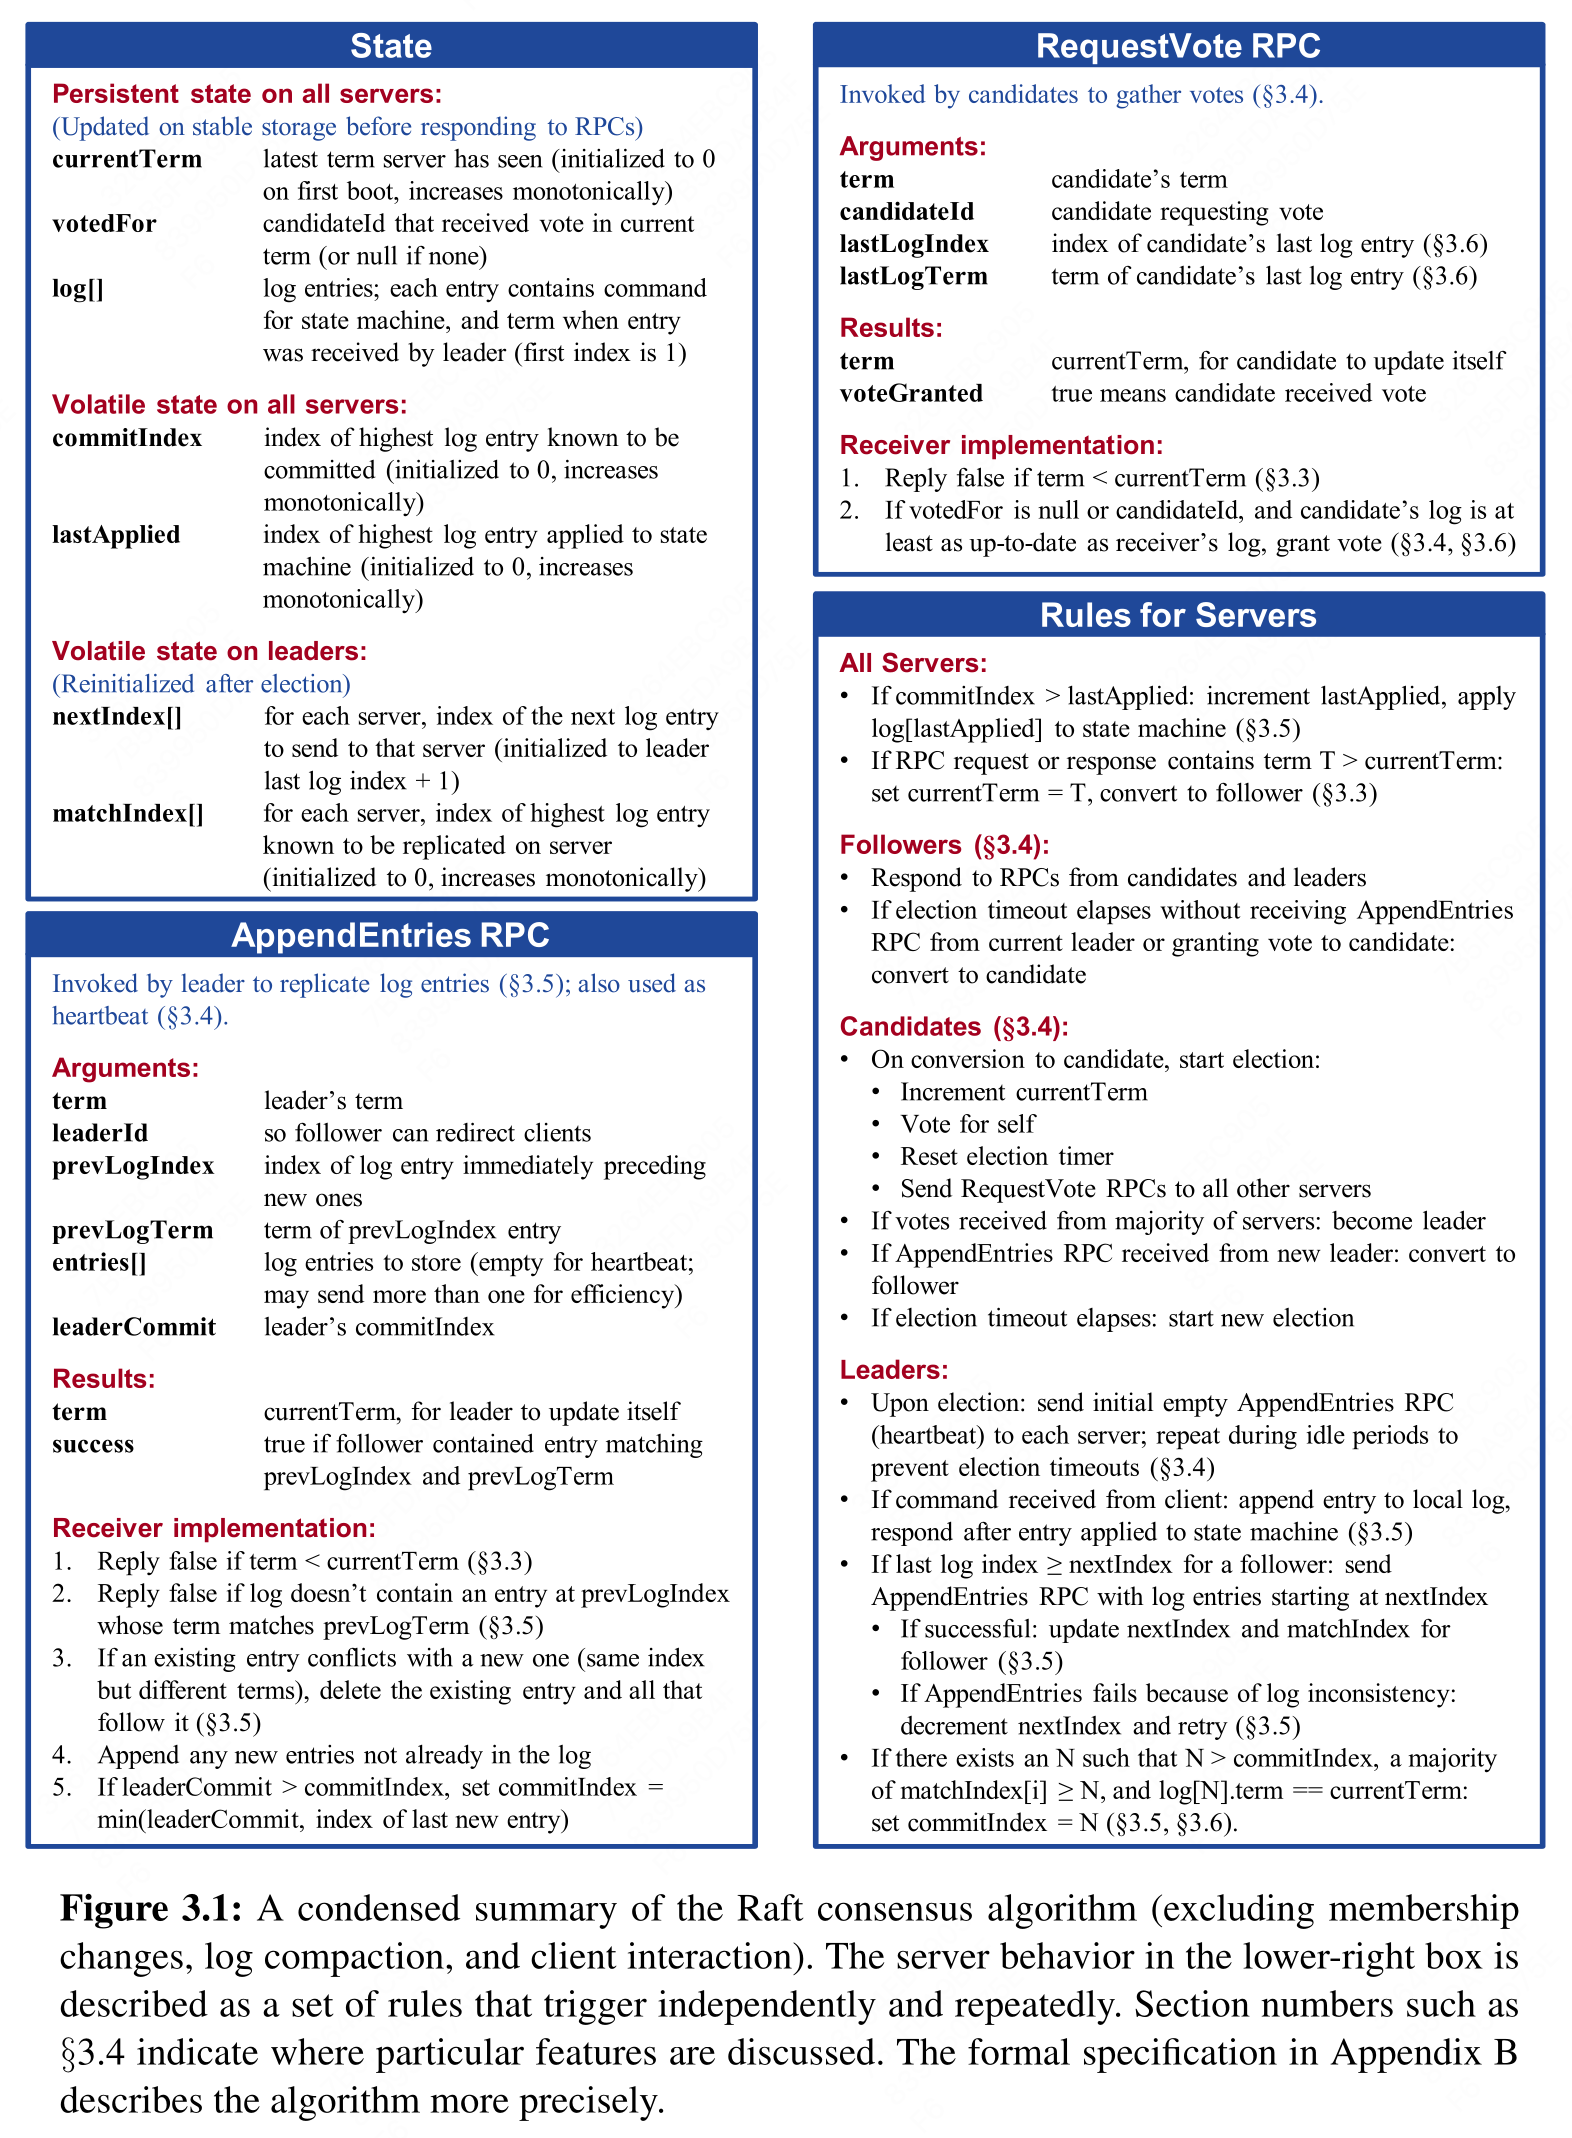
\includegraphics[width=.99\textwidth]{../../images/papers/17.png}
\label{}
\end{center}
Given the leader approach, Raft decomposes the consensus problem into three relatively independent
subproblems:
\begin{itemize}
\item Leader election: a new leader must be chosen when starting the cluster and when an existing leader fails
\item Log replication: the leader must accept log entries from clients and replicate them across the cluster, forcing the other logs to agree with its own
\item Safety: the key safety property for Raft is the State Machine Safety Property
\end{itemize}


Raft \textbf{SAFETY}:
\begin{itemize}
\item \textbf{Election Safty}: At most one leader can be elected in a given term.
\item \textbf{Leader Append-Only}: A leader never overwrites or deletes entries in its log; it only appends new entries.
\item \textbf{Log Matching}: If two logs contain an entry with the same index and term, then the logs are identical
in all entries up through the given index.
\item \textbf{Leader Completeness}: If a log entry is committed in a given term, then that entry will be present in
the logs of the leaders for all higher-numbered terms.
\item \textbf{State Machine Safety}: If a server has applied a log entry at a given index to its state machine, no
other server will ever apply a different log entry for the same index.
\end{itemize}
\subsection{Log replication}
\label{sec:orgbe4aadb}
The leader decides when it is safe to apply a log entry to the state machines; such an entry is called
\textbf{committed}.
\begin{itemize}
\item Raft guarantees that committed entries are durable and will eventually be executed by all of the
available state machines.
\item A log entry is committed once the leader that created the entry has replicated it on a majority of
the servers. This also commits all preceding entries in the leader’s log, including entries created
by previous leaders.
\item The leader keeps track of the highest index it knows to be committed, and it includes that index in
future AppendEntries RPCs (including heartbeats) so that the other servers eventually find out.
\item Once a follower learns that a log entry is committed, it applies the entry to its local state
machine (in log order).
\end{itemize}

Raft maintains the following properties, which together constitute the \textbf{Log Matching Property}:
\begin{itemize}
\item If two entries in different logs have the same index and term, then they store the same command.
\item If two entries in different logs have the same index and term, then the logs are identical in all
preceding entries.

\item The first property follows from the fact that a leader creates at most one entry with a given log
index in a given term, and log entries never change their position in the log.

If two entries have the same term, then they come from the same leader. If a log is replicated into
a specific entry, then the index of that log is the same as the leader. Therefore the two entries
have the same command as they come from the same entry from the same leader in the same term.
\item The second property is guaranteed by a consistency check performed by AppendEntries. When sending an
AppendEntries RPC, the leader includes the \uline{index and term of the entry} in its log that immediately
\uline{precedes} the new entries\wu{(prev log)}. If the follower does not find an entry in its log with the same index and
term, then it refuses the new entries.

The consistency check acts as an induction step: the initial empty state of the logs satisfies the
Log Matching Property, and the consistency check preserves the Log Matching Property whenever logs
are extended. As a result, whenever AppendEntries returns successfully, the leader knows that the
follower’s log is identical to its own log up through the new entries.
\end{itemize}


A follower may be missing entries that are present on the leader, it may have extra entries that are
not present on the leader, or both. Missing and extraneous entries in a log may span multiple terms.
\begin{center}
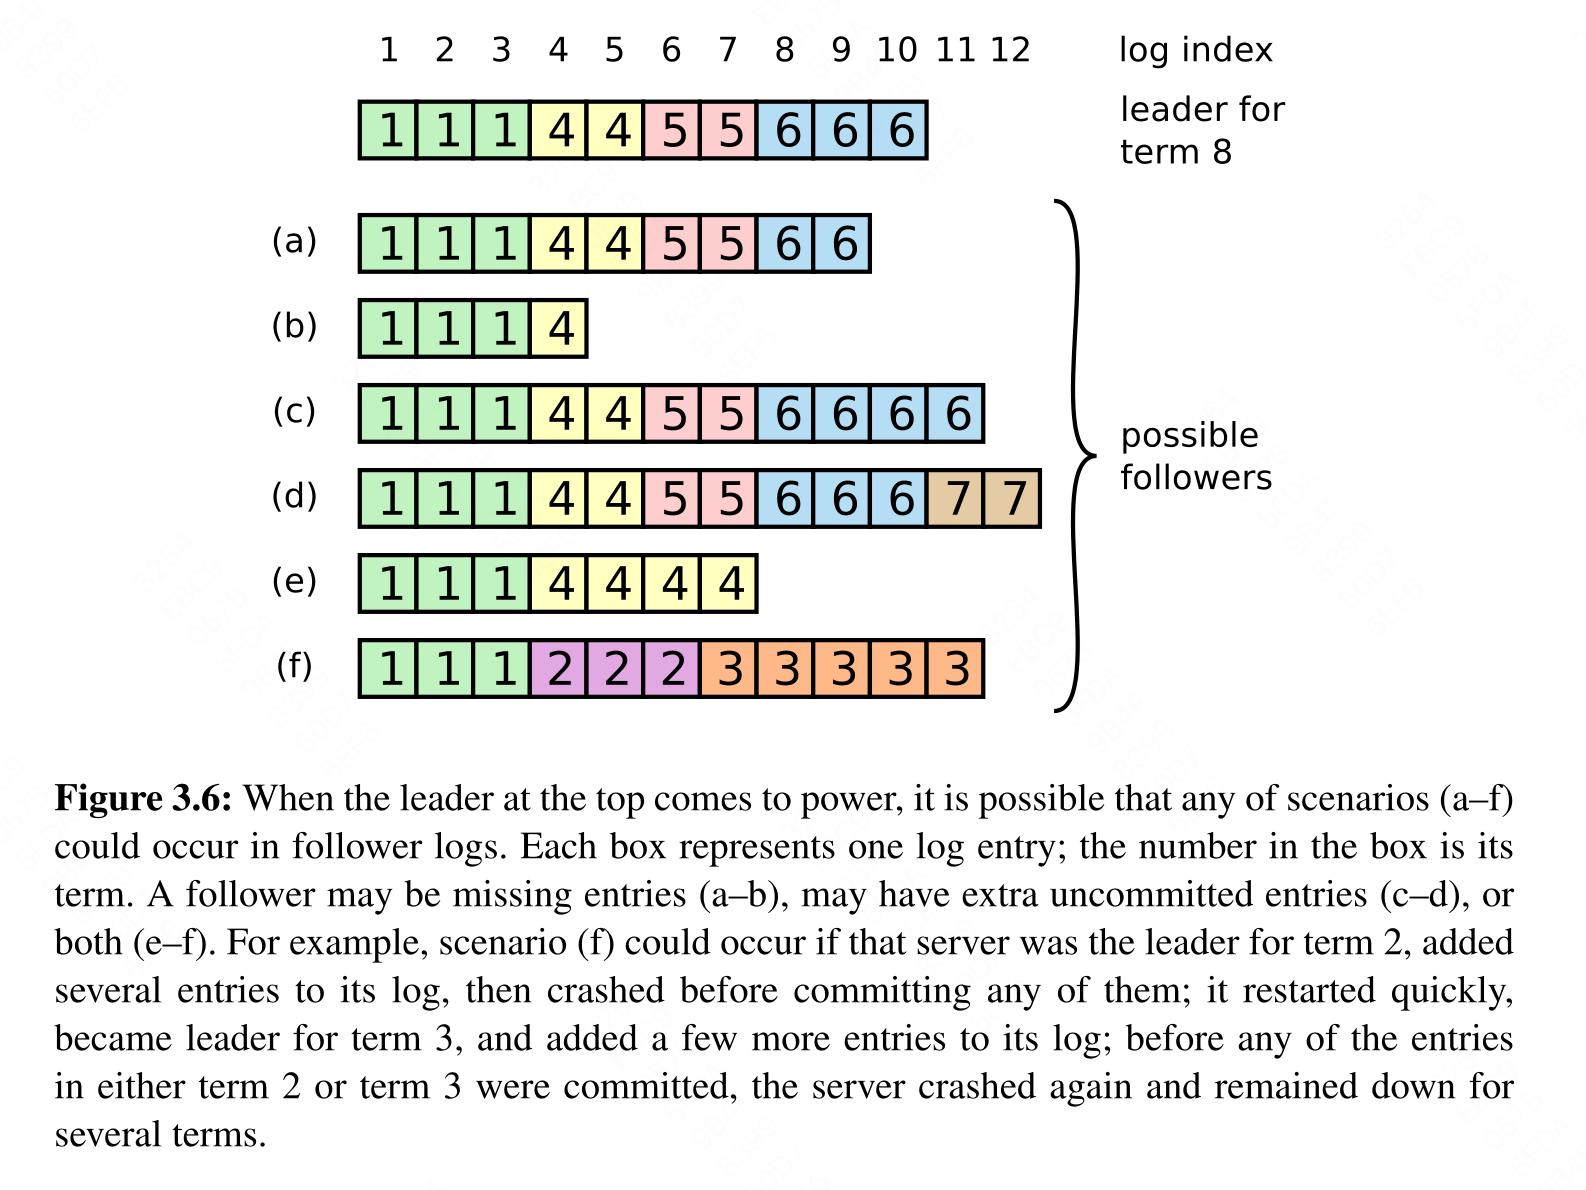
\includegraphics[width=.9\textwidth]{../../images/papers/13.png}
\label{3.6}
\end{center}

The leader handles inconsistencies by forcing the followers’ logs to duplicate its own. This means
that conflicting entries in follower logs will be overwritten with entries from the leader's log.

To bring a follower’s log into consistency with its own, the leader must find the latest log entry
where the two logs agree, delete any entries in the follower’s log after that point, and send the
follower all of the leader’s entries after that point. All of these actions happen in response to the
consistency check performed by AppendEntries RPCs:
\begin{itemize}
\item The leader maintains a \textbf{nextIndex} for each follower, which is the index of the next log entry the leader will send to that follower.
\item When a leader first comes to power, it initializes all nextIndex values to the index just after the
last one in its log.
\item If a follower's log is inconsistent with the leader's, the AppendEntries consistency check will fail
in the next AppendEntries RPC. After a rejection, the leader decrements the follower's nextIndex and
retries the AppendEntries RPC. Eventually the nextIndex will reach a point where the leader and
follower logs match.
\end{itemize}

Until the leader has discovered where it and the follower’s logs match, the leader can send
AppendEntries with no entries (like heartbeats) to save bandwidth. Then, once the matchIndex
immediately precedes the nextIndex, the leader should begin to send the actual entries.

If desired, the protocol can be optimized to reduce the number of rejected AppendEntries RPCs:
\begin{itemize}
\item when rejecting an AppendEntries request, the follower can include the term of the conflicting entry
and the first index it stores for that term. With this information, the leader can decrement
nextIndex to bypass all of the conflicting entries in that term;
\item the leader can use a binary search approach to find the first entry where the follower’s log differs
from its own; this has better worst-case behavior.
\end{itemize}
\subsection{Safty}
\label{sec:org57e5be8}
This section completes the Raft algorithm by adding a restriction on which servers may be elected
leader. The restriction ensures that the leader for any given term contains all of the entries committed in previous terms.
\subsubsection{Election restriction}
\label{sec:org459241d}
In any leader-based consensus algorithm, the leader \textbf{must} eventually store all of the committed log
entries.

Raft uses the voting process to \uline{prevent a candidate from winning an election unless its log contains}
\uline{all committed entries}:
\begin{itemize}
\item A candidate must contact a majority of the cluster in order to be elected, which means that every
committed entry must be present in at least one of those servers.
\item If the candidate's log is at least as \textbf{up-to-date} as any other log in that majority, then it will
hold all the committed entries.
\end{itemize}

Raft determines which of two logs is more \textbf{up-to-date} by comparing the index and term of the last
entries in the logs.
\begin{itemize}
\item If the logs have last entries with different terms, then the log with the later term is more up-to-date.
\item If the logs end with the same term, then whichever log is longer is more up-to-date.
\end{itemize}

The correctness of this notion of up-to-date comes from Log Matching Property.
\subsubsection{Committing entries from previous terms}
\label{sec:org2492c77}
A leader cannot immediately conclude that an entry from a previous term is committed once it is stored
on a majority of servers:
\begin{center}
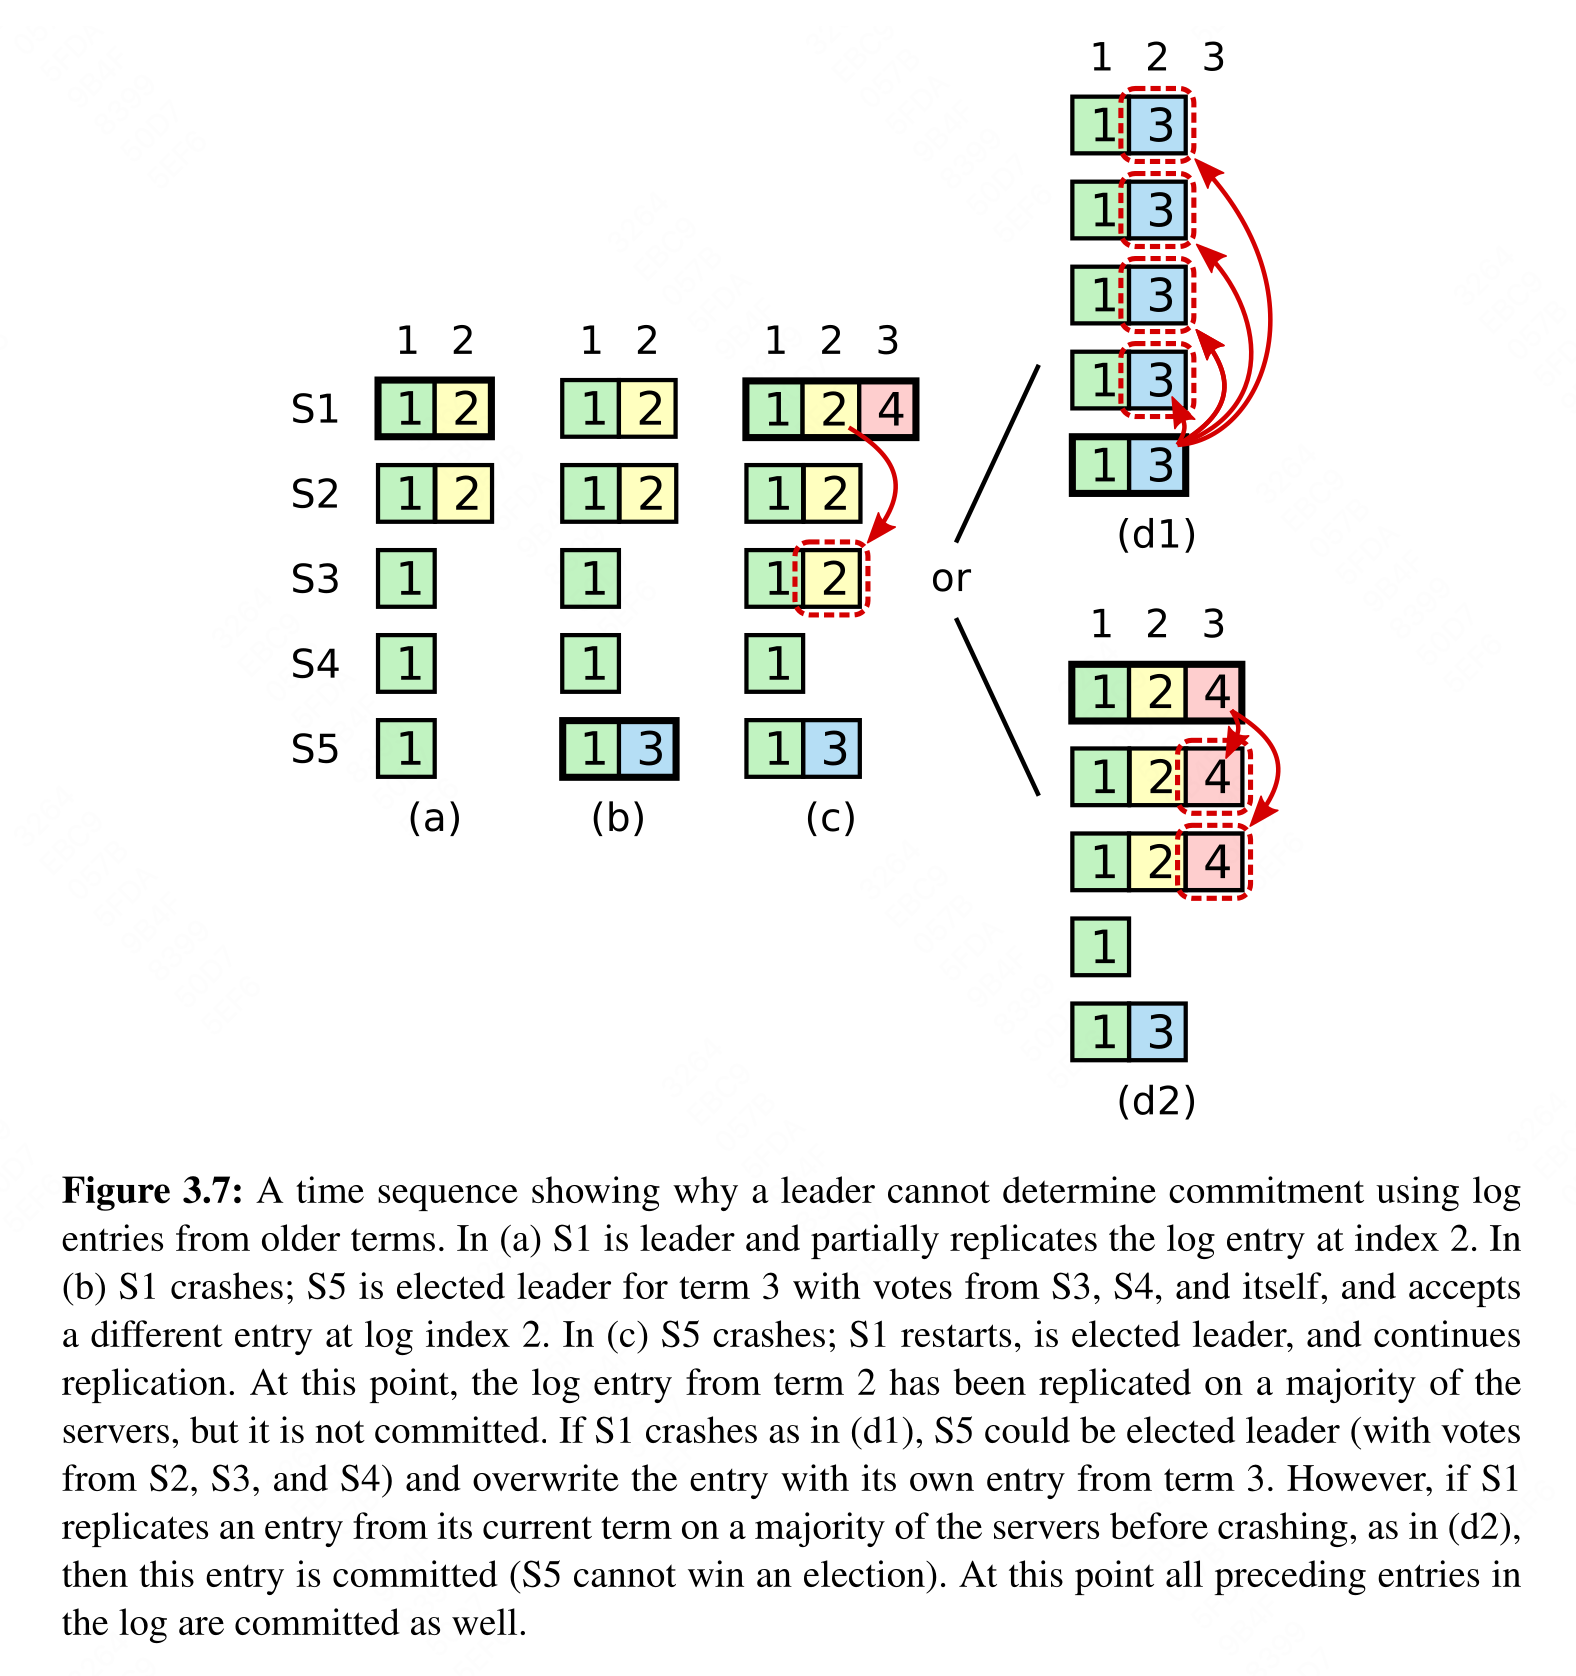
\includegraphics[width=.9\textwidth]{../../images/papers/12.png}
\label{3.7}
\end{center}

To eliminate problems like the one in Figure \ref{3.7}, Raft never commits log entries from previous
terms by counting replicas; once an entry from the current term has been committed in this way, then all prior
entries are committed indirectly because of the Log Matching Property.
\subsubsection{Safety argument}
\label{sec:org80fc364}
\label{3.3}
Assume Leader Completeness Property does not hold. Suppose the leader for term \(T\) \(leader_T\)
commits a log entry from its term, but that log entry is not stored by the leader of some future term.
Consider the smallest term \(U>T\) whose leader \(leader_U\) does not store the entry.
\begin{enumerate}
\item The committed entry must have been absent from \(leader_U\)'s log at the time of its election.
\item \(leader_T\) replicated the entry on a majority of the cluster, and \(leader_U\) received votes
from a majority of the cluster. Thus at least one server both accepted the entry from \(leader_T\)
and voted for \(leader_U\).
\item The voter must have accepted the committed entry from \(leader_T\) \textbf{before} voting for \(leader_U\);
otherwise it would have rejected the AppendEntries request from \(leader_T\)
\item The voter still stored the entry when it voted for \(leader_U\), since every intervening leader
contained the entry, leaders never remove entries, and followers only remove entries if they
conflict with the leader.
\item The voter granted its vote to \(leader_U\), so \(leader_U\)'s log must have been as up-to-date as
the voter's. This leaders to one of two contradictions.
\item First, if the voter and \(leader_U\) shared the same last log term, then \(leader_U\)'s log must
have been at least as long as the voter's, so its log contained every entry in the voter's log.
\item Otherwise, \(leader_U\)'s last log term must have been larger than the voter's. Moreover, it was
larger than \(T\), since the voter's last log term was at least \(T\). The earlier leader that
created \(leader_U\)'s last log entry must have contained the committed entry in its log. Then by
the Log Matching Property, \(leader_U\)'s log must also contain the committed entry, which is a contradiction.
\item Thus, the leaders of all terms greater than \(T\) must contain all entries from term \(T\) that are
committed in term \(T\).
\item The Log Matching Property guarantees that future leaders will also contain entries that are
committed indirectly.
\end{enumerate}



Given the Leader Completeness Property, we can prove the State Machine Safety Property from, which
states that if a server has applied a log entry at a given index to its state machine, no other server
will ever apply a different log entry for the same index:
\begin{itemize}
\item At the time a server applies a log entry to its state machine, its log must be identical to the
leader’s log up through that entry, and the entry must be committed. Now consider the lowest term in
which any server applies a given log index; the Leader Completeness Property guarantees that the
leaders for all higher terms will store that same log entry, so servers that apply the index in
later terms will apply the same value. Thus, the State Machine Safety Property holds.
\end{itemize}


Finally, Raft requires servers to apply entries in log index order. Combined with the State Machine
Safety Property, this means that all servers will apply exactly the same set of log entries to their
state machines, in the same order.
\subsubsection{Followe rand candidate crashes}
\label{sec:orgb3791b1}
\subsubsection{Persisted state and server restarts}
\label{sec:org8b92ded}
\begin{itemize}
\item current term and vote: prevent the server from voting twice \wu{means vote for different candidates}
in the same term or replacing log entries from a newer leader with those from a deposed
leader\wu{term}.
\item new log entries before they are committed: prevents committed entries from being lost or
“uncommitted” when servers restart.
\item \emph{last applied} index
\end{itemize}
\subsubsection{Timing and availability}
\label{sec:org23f328d}
\subsubsection{Leadership transfer extention}
\label{sec:org79def38}
To transfer leadership in Raft, the prior leader sends its log entries to the target server, then the
target server runs an election without waiting for the election timeout to elaspe.
\begin{enumerate}
\item The prior leader stops accepting new client requests.
\item The prior leader fully updates the target server's log to match its own, using the normal log
replication mechanism
\item The prior leader sends a \emph{TimeoutNow} request to the target server.
\end{enumerate}

Once the target server receives the TimeoutNow request, it is highly likely to start an election
before any other server and become leader in the next term. Its next message to the prior leader will
include its new term number, causing the prior leader to step down. At this point, leadership transfer
is complete.

It is also possible for the target server to fail; in this case, the cluster must resume client
operations. If leadership transfer does not complete after about an election timeout, the prior leader
aborts the transfer and resumes accepting client requests. If the prior leader was mistaken and the
target server is actually operational, then at worst this mistake will result in an extra election,
after which client operations will be restored.
\section{Cluster membership changes}
\label{sec:orgd9da6e7}
\begin{center}
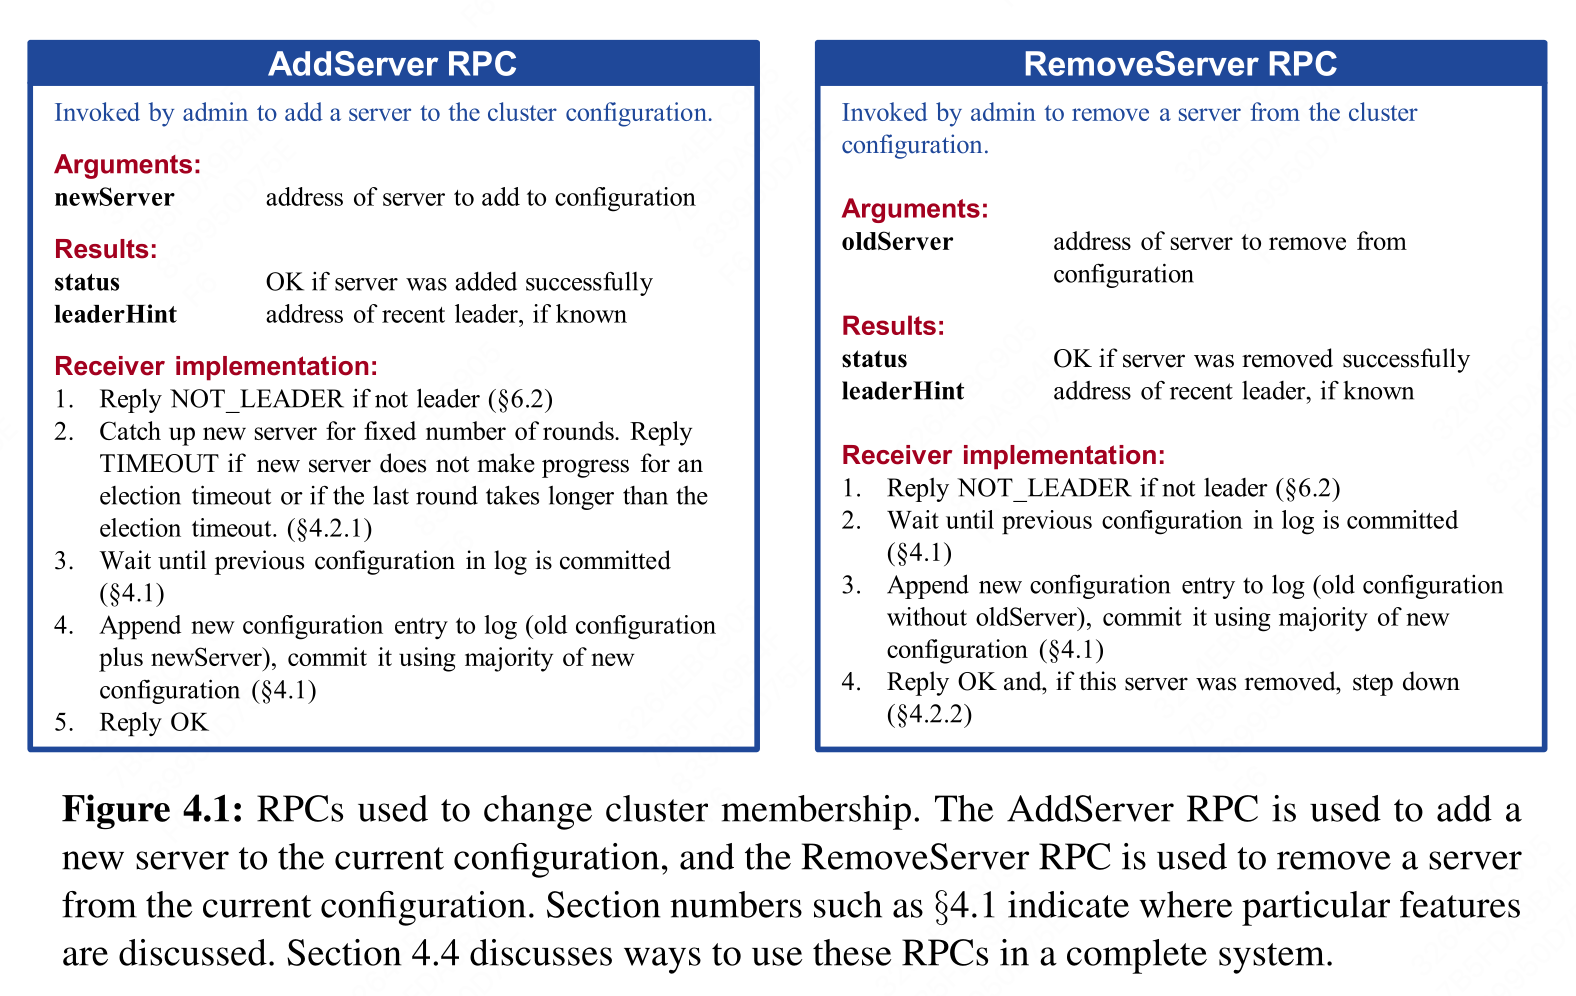
\includegraphics[width=.99\textwidth]{../../images/papers/14.png}
\label{}
\end{center}
\subsection{Safety}
\label{sec:org43557f7}
\begin{itemize}
\item Goal: no point during the transition where it is possible for two leaders to be elected for the same term.
\item Difficulty: it isn’t possible to atomically switch all of the servers at once, so the cluster can
potentially split into two independent majorities during the transition
\begin{center}
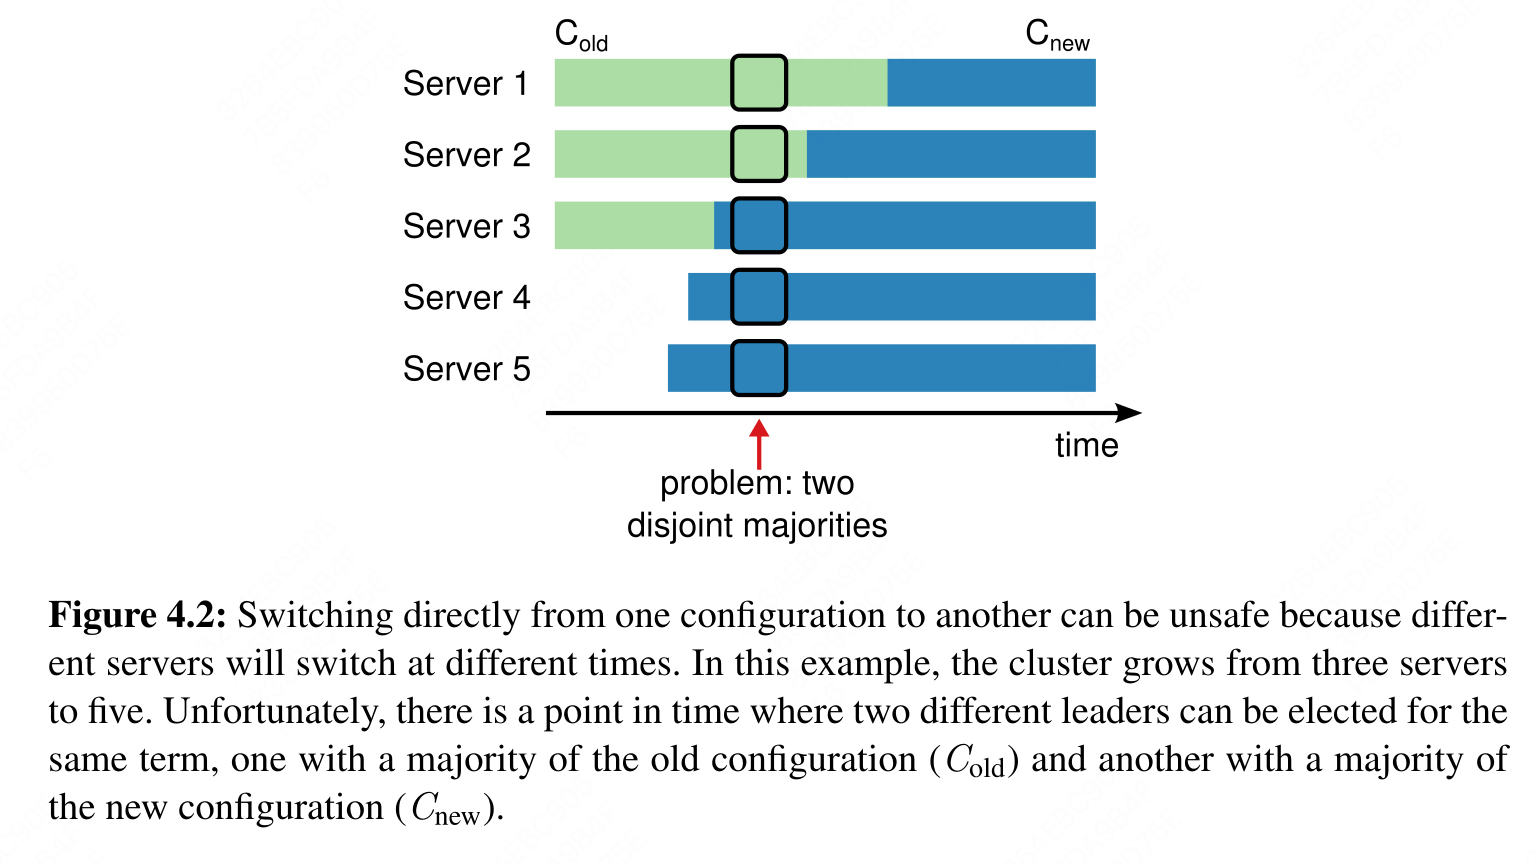
\includegraphics[width=.99\textwidth]{../../images/papers/15.png}
\label{4.2}
\end{center}
\end{itemize}

Raft restricts the types of changes that are allowed: only one server can be added or removed from the
cluster at a time. More complex changes in membership are implemented as a series of single-server
changes.

When adding a single server to a cluster or removing a single server from a cluster, any majority of
the old cluster overlaps with any majority of the new cluster. This overlap prevents the cluster from
splitting into two independent majorities; in terms of the safety argument of Section \ref{3.3}, it
guarantees the existence of “the voter”. Thus, when adding or removing just a single server, it is
safe to switch directly to the new configuration.

\begin{center}
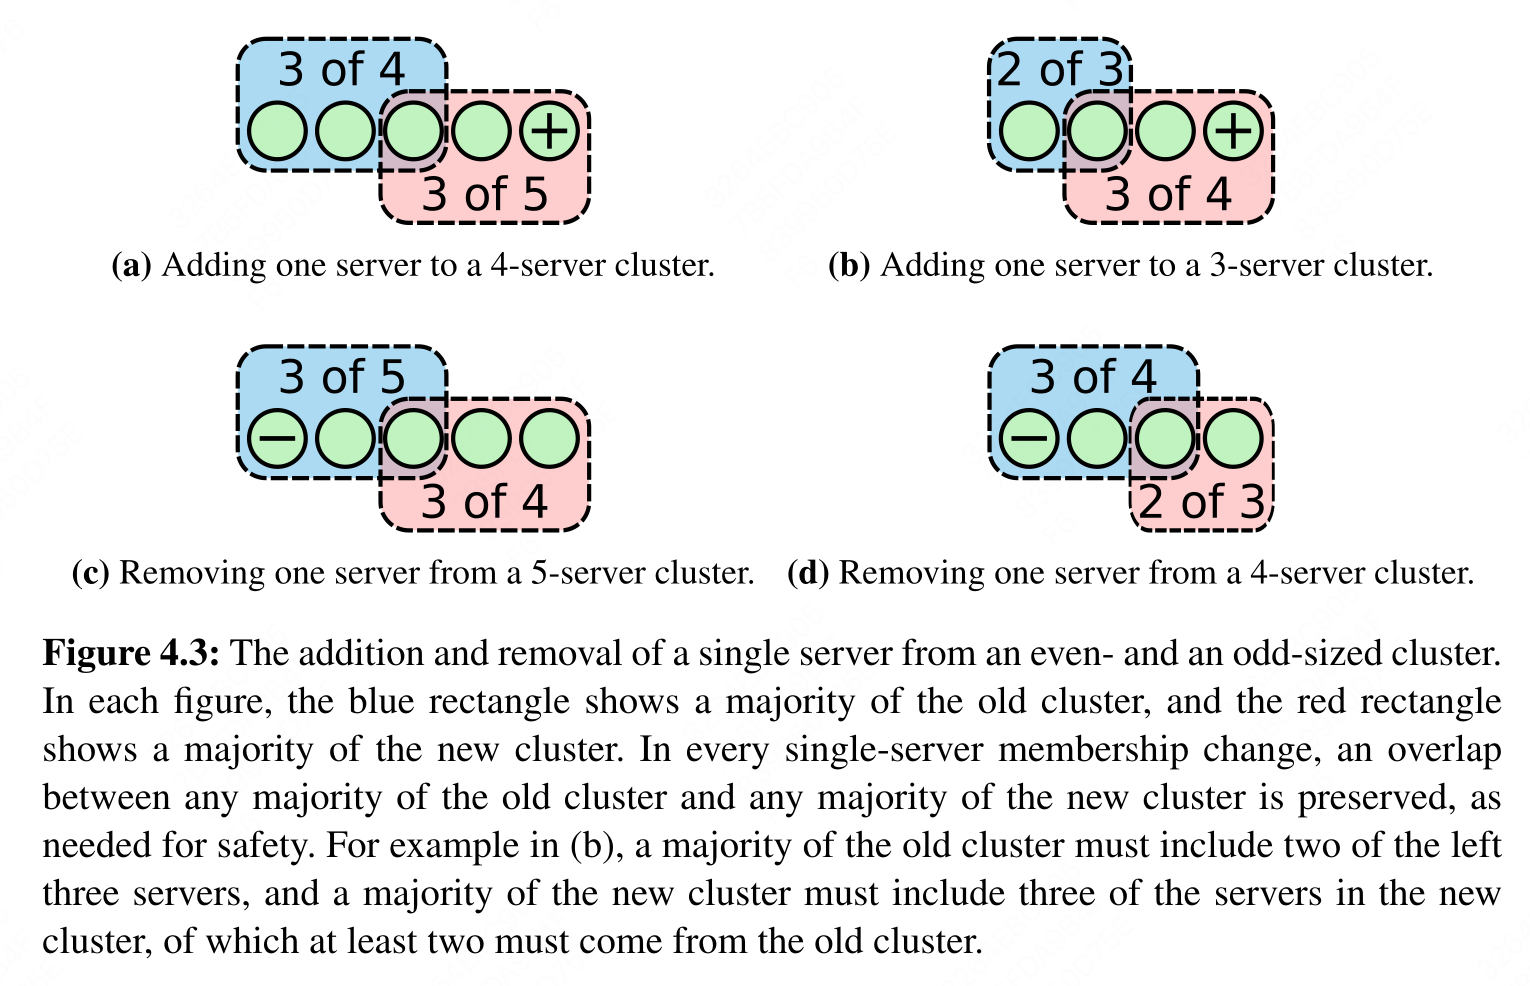
\includegraphics[width=.99\textwidth]{../../images/papers/16.png}
\label{}
\end{center}

When the leader receives a request to add or remove a server from its current configuration
\(C_{old}\), it appends the new configuration \(C_{new}\)  as an entry in its log and replicates that
entry using the normal Raft mechanism. The new configuration takes effect on each server as soon as it
is added to that server’s log: the \(C_{new}\) entry is replicated to the \(C_{new}\) servers, and a majority of the new
configuration is used to determine the \(C_{new}\) entry’s commitment.

The configuration change is complete once the \(C_{new}\) entry is committed. At this point, the leader knows
that a majority of the \(C_{new}\) servers have adopted \(C_{new}\) . It also knows that any servers that have not
moved to \(C_{new}\) can no longer form a majority of the cluster, and servers without \(C_{new}\) cannot be elected
leader. Commitment of \(C_{new}\) allows three things to continue:
\begin{enumerate}
\item The leader can acknowledge the successful completion of the configuration change.
\item If the configuration change removed a server, that server can be shut down.
\item Further configuration changes can be started. Before this point, overlapped configuration changes
could degrade to unsafe situations as in Fig \ref{4.2}
\end{enumerate}



\begin{itemize}
\item \uline{Servers always use the latest configuration in their logs, regardless of whether that configuration}
\uline{entry has been committed.} This allows leaders to easily avoid overlapping configuration changes (the
third item above), by not beginning a new change until the previous change’s entry has committed.
\item It is only safe to start another membership change once a majority of the old cluster has moved to
operating under the rules of \(C_{new}\). If servers adopted \(C_{new}\) only when they learned that \(C_{new}\)
was committed, Raft leaders would have a difficult time knowing when a majority of the old cluster
had adopted it.
\end{itemize}


In Raft, it is the caller’s configuration that is used in reaching consensus, both for voting and for log replication:
\begin{itemize}
\item A server accepts \texttt{AppendEntries} requests from a leader that is not part of the server’s latest
configuration. Otherwise, a new server could never be added to the cluster (it would never accept any log entries preceding the configuration entry that adds the server).
\item \uline{A server also grants its vote to a candidate that is not part of the server’s latest configuration}
(if the candidate has a sufficiently up-to-date log and a current term). This vote may occasionally
be needed to keep the cluster available. For example, consider adding a fourth server to a
three-server cluster. If one server were to fail, the new server’s vote would be needed to form a
majority and elect a leader.
\end{itemize}

Thus, servers process incoming RPC requests without consulting their current configurations.
\subsection{Availability}
\label{sec:orgc76fa2f}
\subsubsection{Catching up new servers}
\label{sec:org944db65}
When a server is added to the cluster, it typically will not store any log entries. If it is added to
the cluster in this state, its log could take quite a while to catch up to the leader’s, and during
this time, the cluster is more vulnerable to unavailability:
\begin{itemize}
\item A three-server cluster can normally tolerate one failure with no loss in availability. However, if a
fourth server with an empty log is added to the same cluster and one of the original three servers
fails, the cluster will be temporarily unable to commit new entries (\ref{4.4} (a)).
\item Many new servers are added to a cluster in quick succession, where the new servers are needed to
form a majority of the cluster (\ref{4.4} (b)).
\end{itemize}

\begin{center}
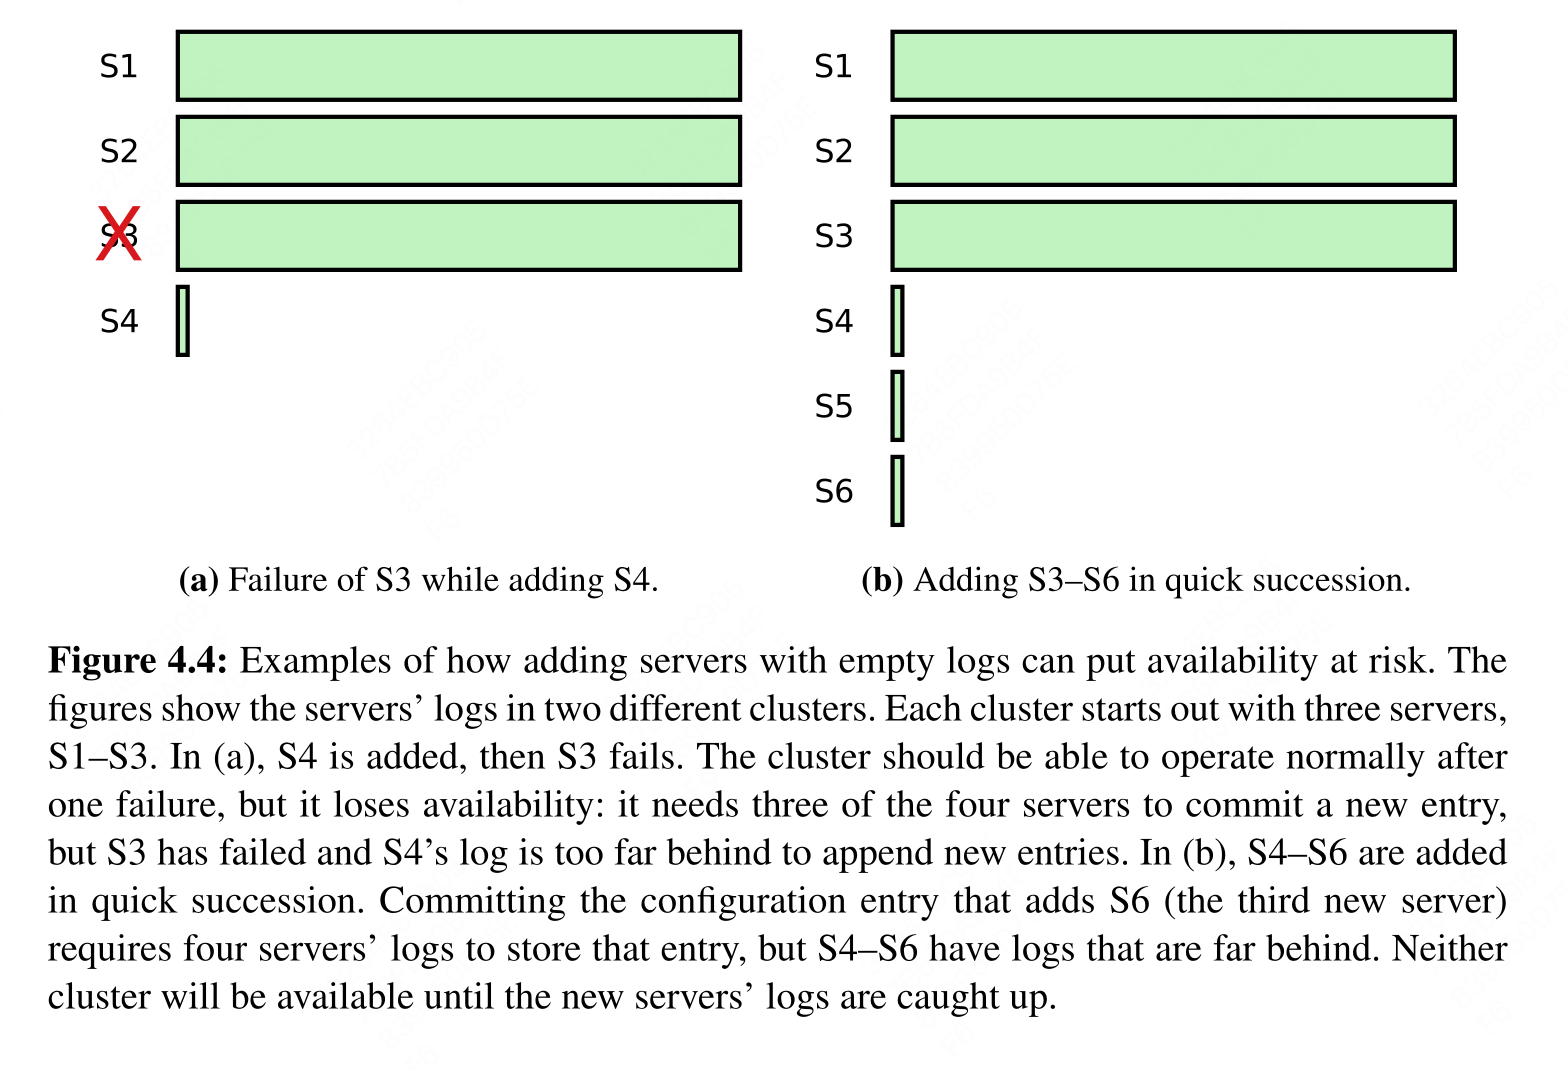
\includegraphics[width=.99\textwidth]{../../images/papers/18.png}
\label{4.4}
\end{center}

In order to avoid availability gaps, Raft introduces an additional phase before the configuration
change, in which a new server joins the cluster as a \textbf{non-voting member}. The leader replicates log
entries to it, but it is not yet counted towards majorities for voting or commitment purposes. Once
the new server has caught up with the rest of the cluster, the reconfiguration can proceed as
described above. (The mechanism to support non-voting servers can also be useful in other contexts;
for example, it can be used to replicate the state to a large number of servers, which can serve
read-only requests with relaxed consistency.)

We suggest the following algorithm to determine when a new server is sufficiently caught up to add to
the cluster:
\begin{itemize}
\item The replication of entries to the new server is split into rounds, as shown in Figure \ref{4.5}.
\item Each round replicates all the log entries present in the leader’s log at the start of the round to
the new server’s log. While it is replicating entries for its current round, new entries may arrive
at the leader; it will replicate these during the next round. As progress is made, the round
durations shrink in time.
\item The algorithm waits a fixed number of rounds (such as 10). If the last round lasts less than an
election timeout, then the leader adds the new server to the cluster, under the assumption that
there are not enough unreplicated entries to create a significant availability gap.
\item Otherwise, the leader aborts the configuration change with an error. The caller may always try again
(it will be more likely to succeed the next time, since the new server’s log will already be
partially caught up).
\end{itemize}

\begin{center}
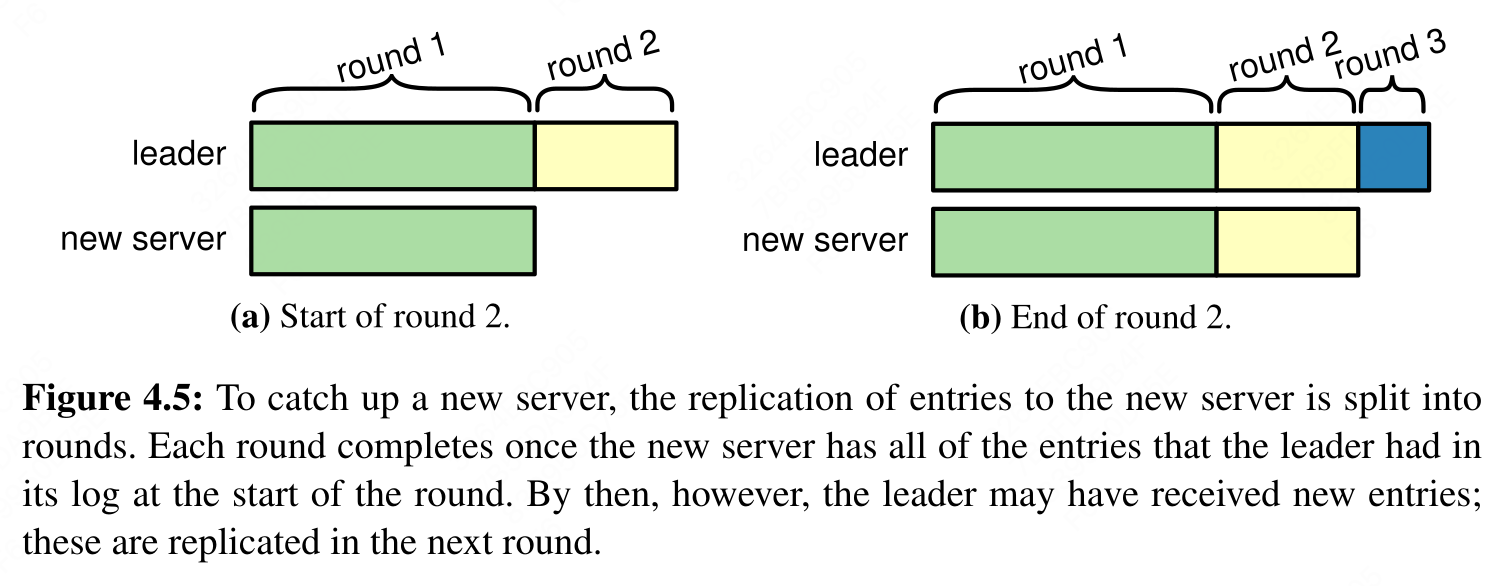
\includegraphics[width=.99\textwidth]{../../images/papers/19.png}
\label{4.5}
\end{center}
\subsubsection{Removing the current leader}
\label{sec:orgac8cb1e}
\subsubsection{Disruptive servers}
\label{sec:orgebde0c5}
Without additional mechanism, servers not in \(C_{new}\) can disrupt the cluster.
\begin{itemize}
\item Once the cluster leader has created the \(C_{new}\) entry, a server that is not in \(C_{new}\) will
no longer receive heartbeats, so it will time out and start new elections.
\item Furthermore, it will not receive the \(C_{new}\) entry or learn of that entry’s commitment, so it
will not know that it has been removed from the cluster. The server will send \texttt{RequestVote} RPCs with
new term numbers, and this will cause the current leader to revert to follower state.
\item A new leader from \(C_{new}\) will eventually be elected, but the disruptive server will time out
again and the process will repeat, resulting in poor availability. If multiple servers have been
removed from the cluster, the situation could degrade further.
\end{itemize}


First idea was that, if a server is going to start an election, it would first check that it wouldn't
be wasting everyone's time - that it had a chance to win the election. This introduced a new phase to
elections, called the \textbf{Pre-Vote phase}. A candidate would first ask other servers whether its log was
up-to-date enough to get their vote. Only if the candidate believed it could get votes from a majority
of the cluster would it increment its term and start a normal election.

Unfortunately, the Pre-Vote phase does not solve the problem of disruptive servers: there are
situations where the disruptive server’s log is sufficiently up-to-date, but starting an election
would still be disruptive. Perhaps surprisingly, these can happen even before the configuration change
completes.

\begin{center}
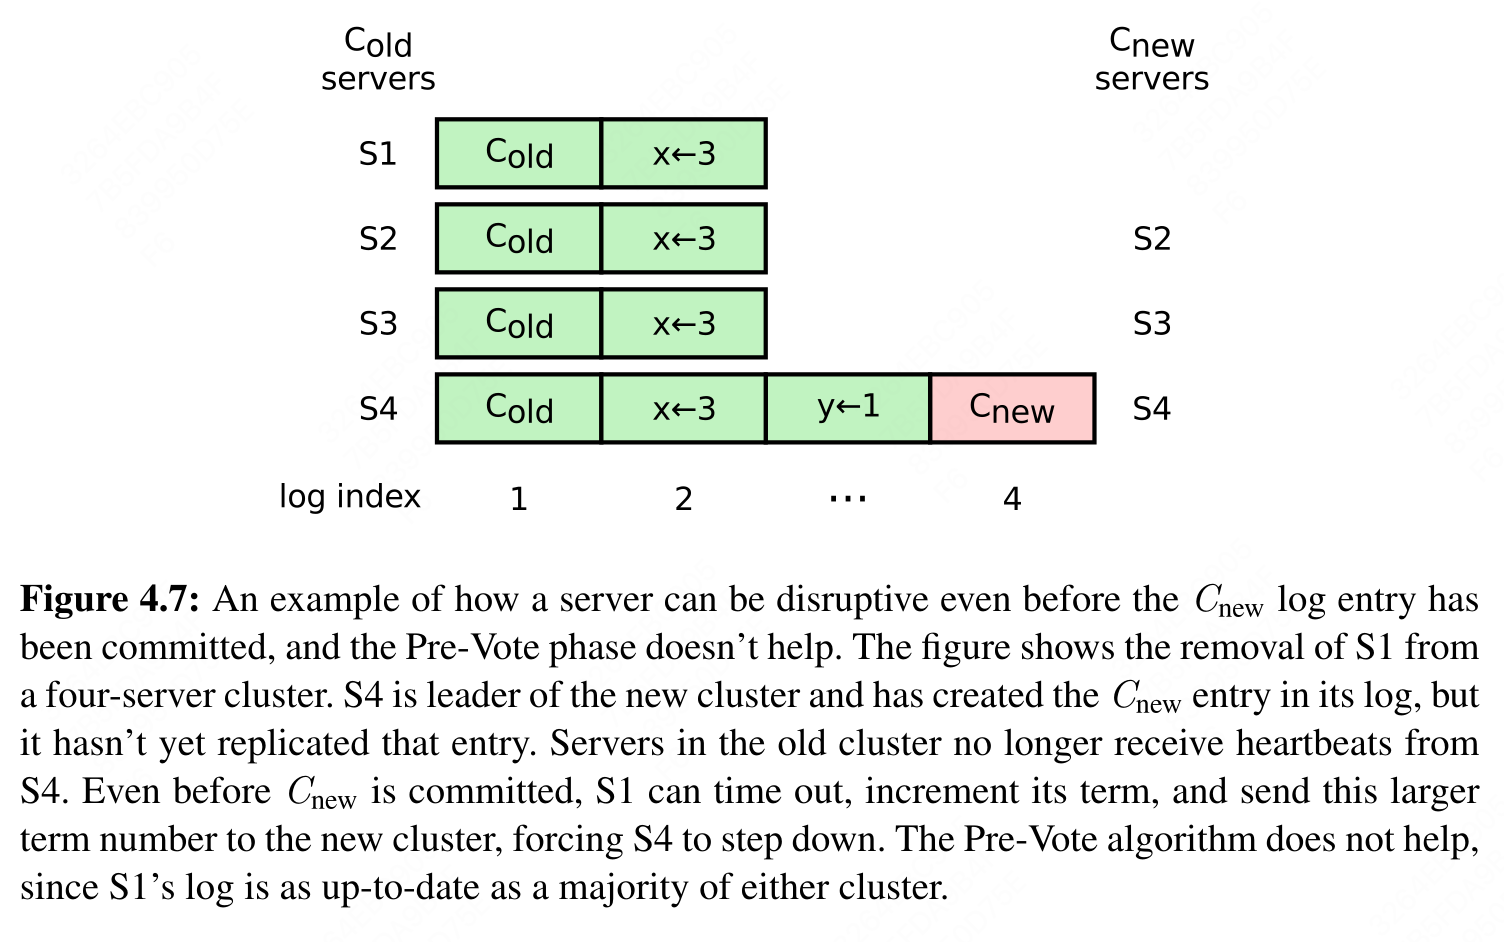
\includegraphics[width=.99\textwidth]{../../images/papers/20.png}
\label{}
\end{center}


Raft’s solution uses heartbeats to determine when a valid leader exists. We modify the \texttt{RequestVote} RPC
to achieve this: if a server receives a \texttt{RequestVote} request within the minimum election timeout of
hearing from a current leader, it does not update its term or grant its vote. It can either drop the
request, reply with a vote denial, or delay the request; the result is essentially the same. This does
not affect normal elections, where each server waits at least a minimum election timeout before
starting an election. However, it helps avoid disruptions from servers not in \(C_{new}\) : while a leader is
able to get heartbeats to its cluster, it will not be deposed by larger term numbers. \label{Problem1}
\subsubsection{Availability}
\label{sec:org8623771}
\label{Problem2}
We show that the algorithm will be able to maintain and replace leaders during membership changes and
that the leader(s) will both service client requests and complete the configuration changes. We
assume, among other things, that a majority of the old configuration is available (at least until \(C_{new}\)
is committed) and that a majority of the new configuration is available.

\begin{enumerate}
\item A leader can be elected at all steps of the configuration change:
\begin{itemize}
\item If the available server with the most up-to-date log in the new cluster has the \(C_{new}\)
entry, it can collect votes from a majority of \(C_{new}\) and become leader
\item Otherwise, the \(C_{new}\) entry must not yet be committed. The available server with the most
up-to-date log among both the old and new clusters can collect votes from a majority of
\(C_{old}\) and a majority of \(C_{new}\), so no matter which configuration it uses, it can
become leader.
\end{itemize}
\end{enumerate}
\section{Log compaction}
\label{sec:org1ed09e3}
\begin{center}
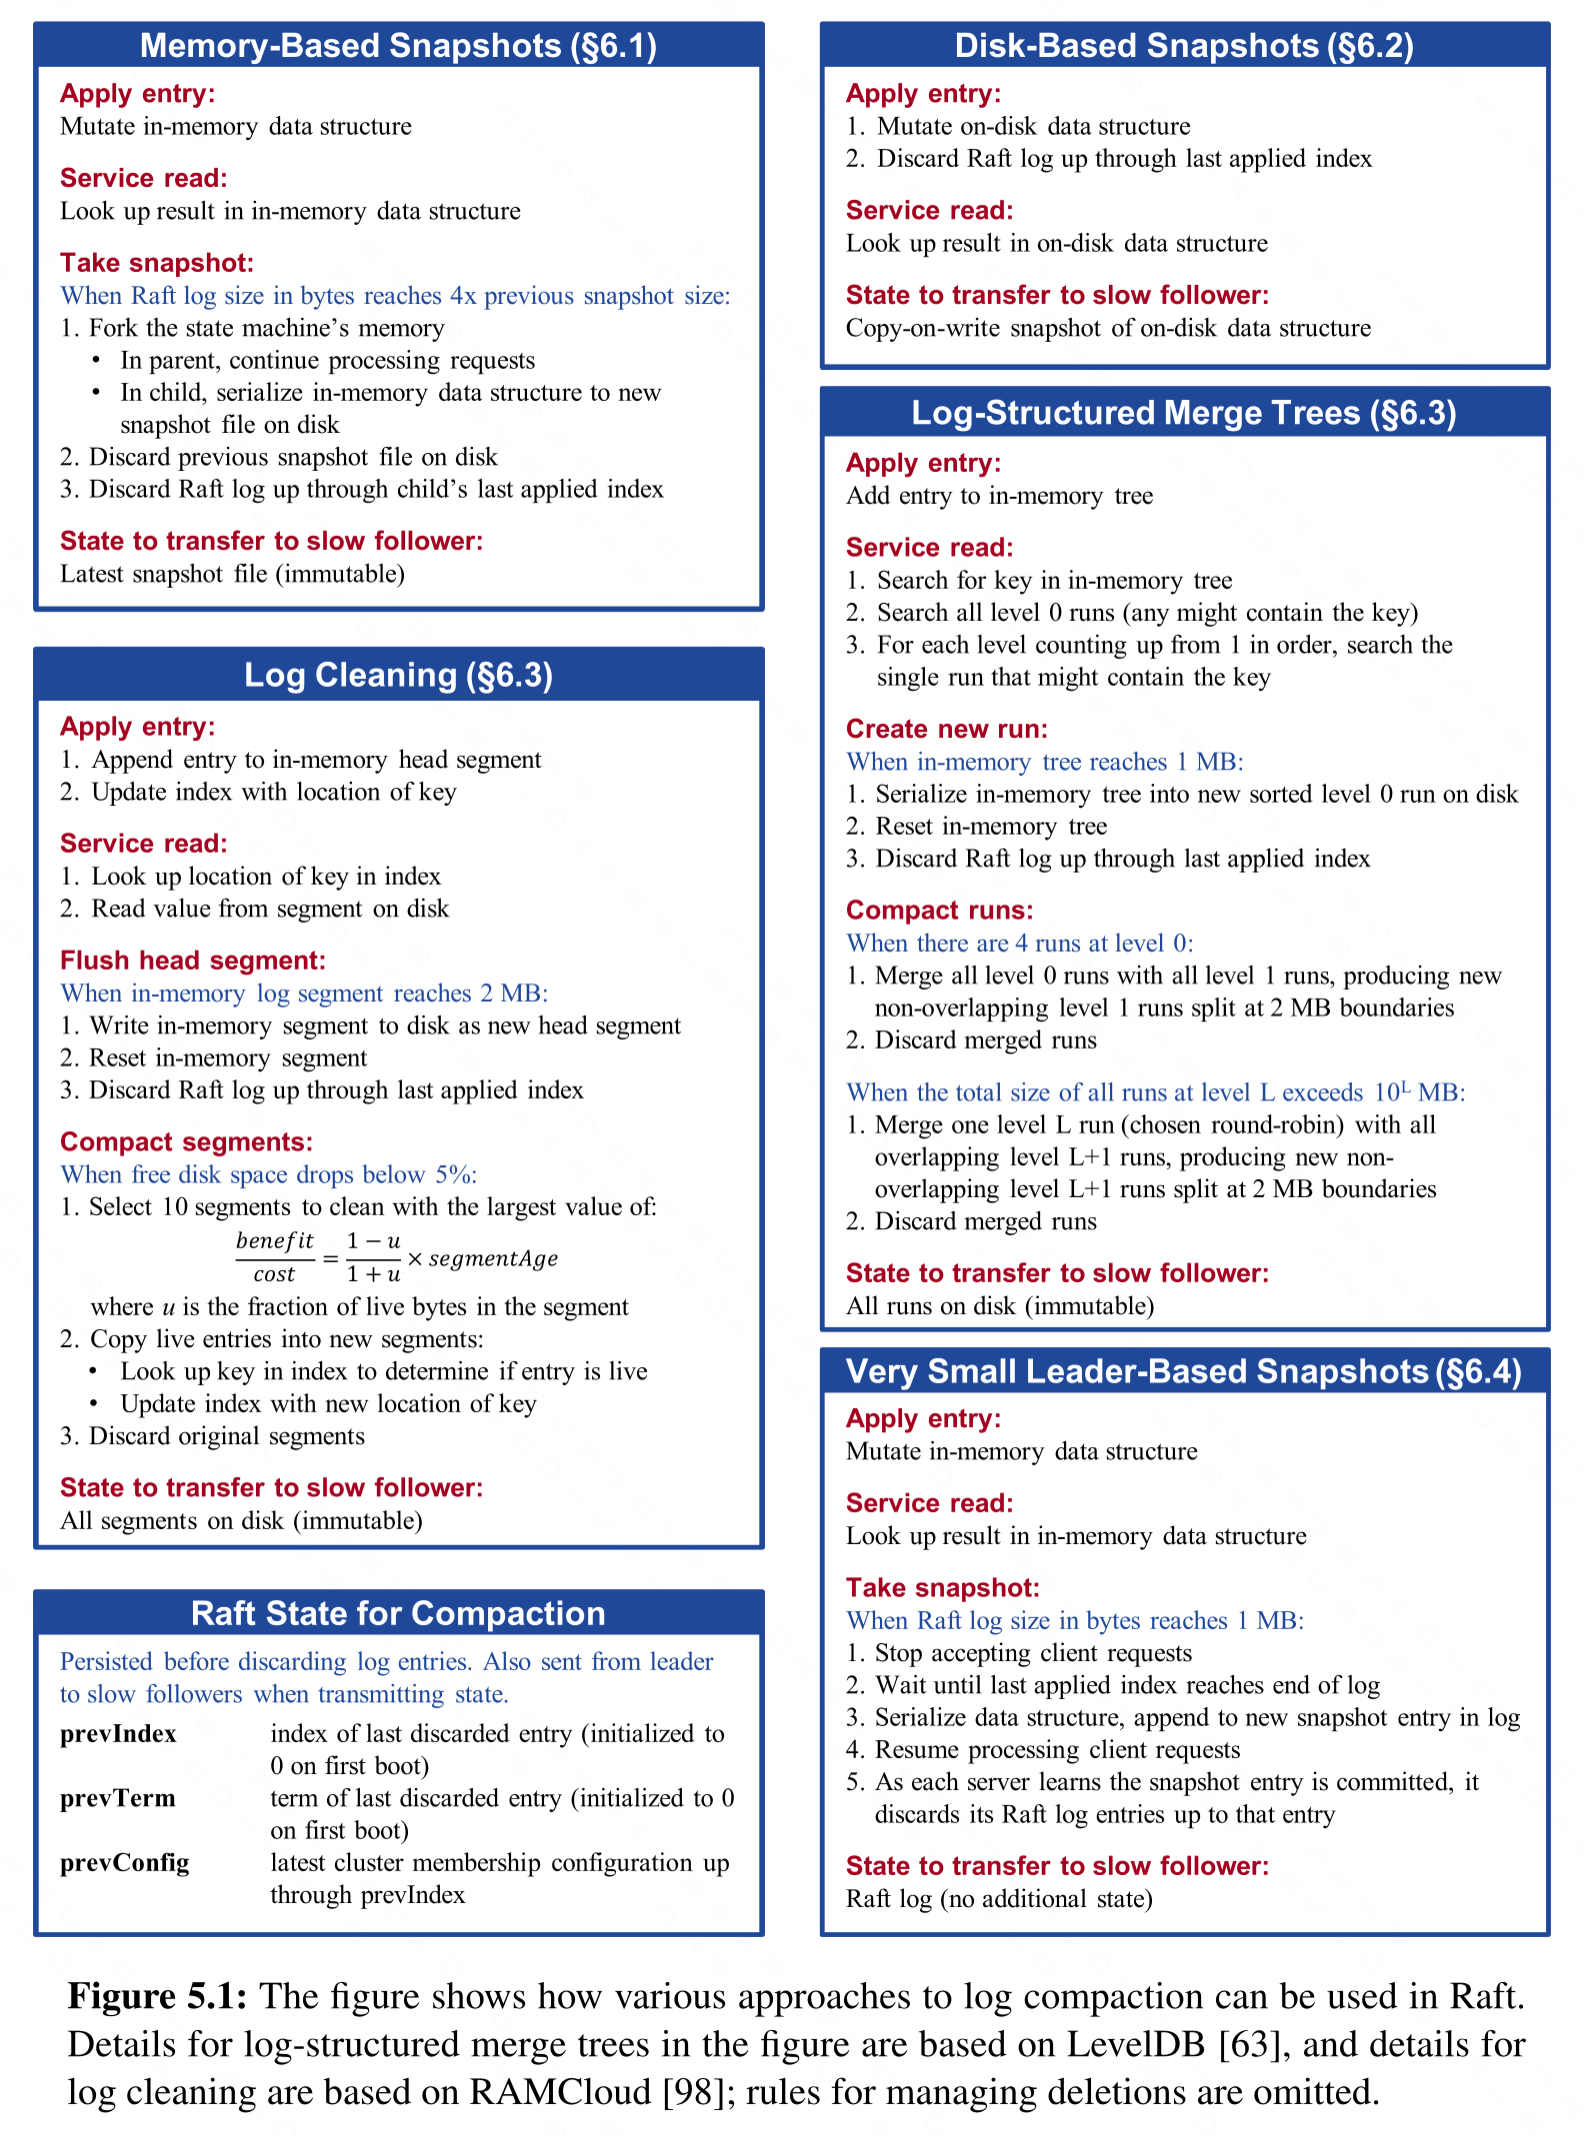
\includegraphics[width=.99\textwidth]{../../images/papers/23.png}
\label{}
\end{center}

The various approaches to compaction share several core concepts.
\begin{itemize}
\item Instead of centralizing compaction decisions on the leader, each server compacts the committed
prefix of its log independently.
\item The basic interaction between the state machine and Raft involves transferring responsibility for a
prefix of the log from Raft to the state machine.
\item Once Raft has discarded a prefix of the log, the state machine takes on two new responsibilities.
\begin{enumerate}
\item If the server restarts, the state machine will need to load the state corresponding to the
discarded log entries from disk before it can apply any entries from the Raft log.
\item the state machine may need to produce a consistent image of the state so that it can be sent to a
slow follower.
\end{enumerate}
It is not feasible to defer compaction until log entries have been “fully replicated” to every
member in the cluster, since a minority of slow followers must not keep the cluster from being
fully available, and new servers can be added to the cluster at any time.
\end{itemize}
\subsection{Snapshotting memory-based state machines}
\label{sec:org93b5ad1}
\subsection{Snapshotting disk-based state machines}
\label{sec:orgf9ed8f2}
Disk-based state machines must be able to provide a consistent snapshot of the disk for the purpose of
transmitting it to slow followers.
\section{Client Interaction}
\label{sec:orgc6fa17a}
\begin{center}
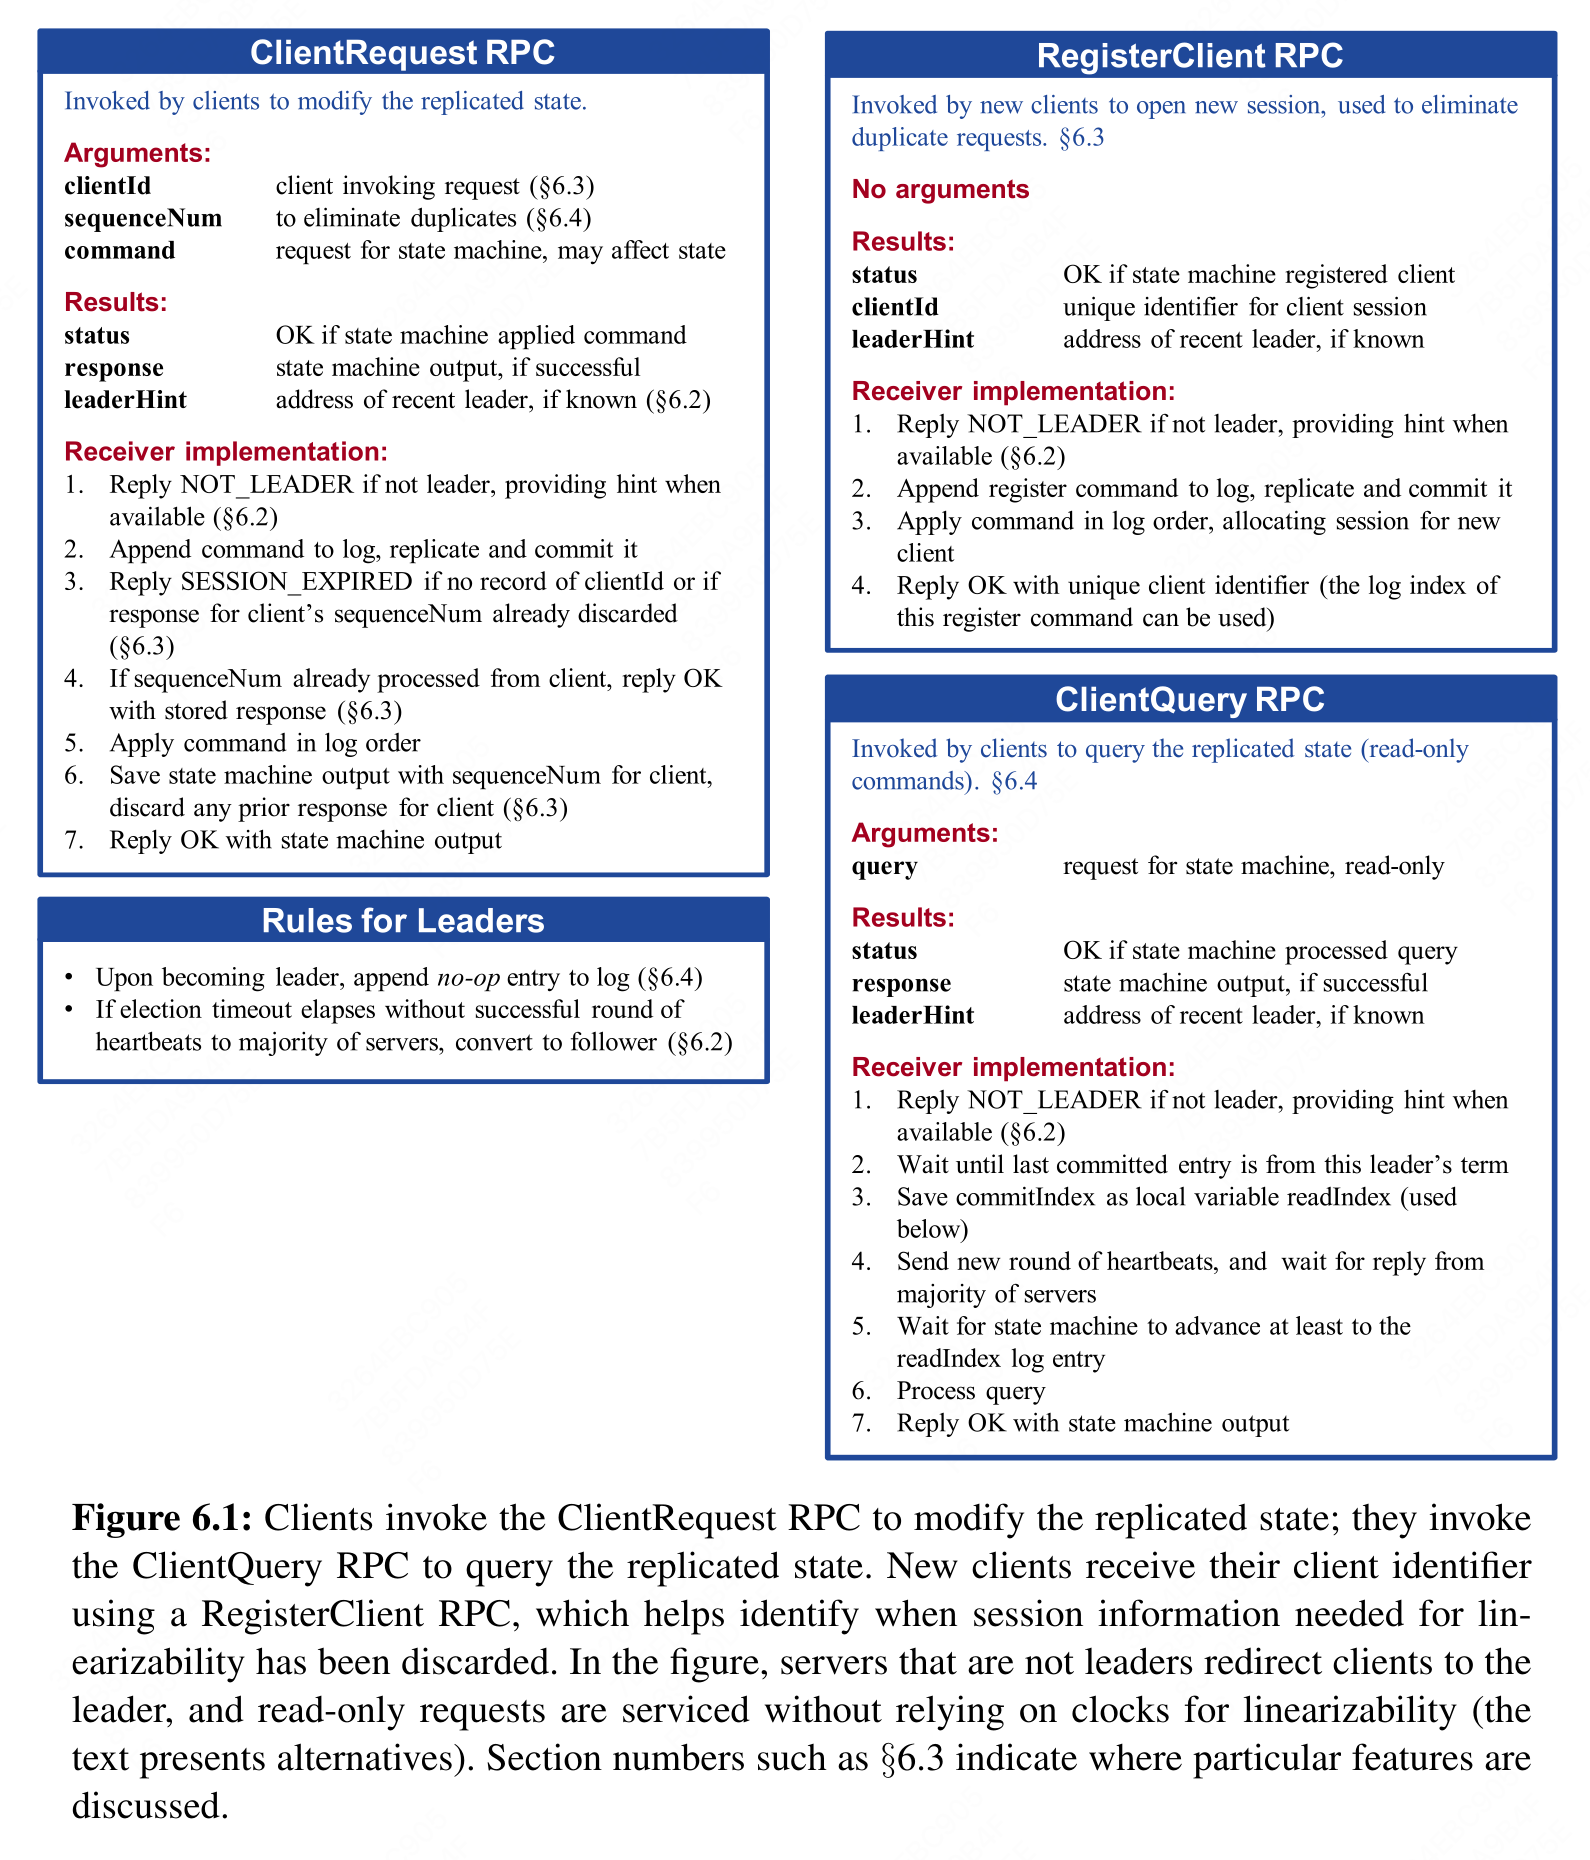
\includegraphics[width=.99\textwidth]{../../images/papers/21.png}
\label{}
\end{center}
\subsection{Finding the cluster}
\label{sec:org49ffd5f}
Two general approaches:
\subsection{Routing requests to the leader}
\label{sec:org26b18ae}
\subsection{Implementing linearizable semantics}
\label{sec:org0a3791d}
Raft provides at-least-once semantics for clients; the replicated state machine may apply a command
multiple times.

In linearizability, each operation appears to execute instantaneously, exactly once, at some point
between its invocation and its response.

To achieve linearizability in Raft, servers must filter out duplicate requests. The basic idea is that
servers save the results of client operations and use them to skip executing the same request multiple
times. To implement this, each client is given a unique identifier, and clients assign unique serial
numbers to every command.

Given this filtering of duplicate requests, Raft provides linearizability. The Raft log provides a
serial order in which commands are applied on every server. Commands take effect instantaneously and
exactly once according to their first appearance in the Raft log, since any subsequent appearances are
filtered out by the state machines as described above.
\subsection{Processing read-only queries more efficiently}
\label{sec:orga12116c}
Fortunately, it is possible to bypass the Raft log for read-only queries and still preserve
linearizability. To do so, the leader takes the following steps:
\begin{enumerate}
\item If the leader has not yet marked an entry from its current term committed, it waits until it has
done so. The Leader Completeness Property guarantees that a leader has all committed entries, but
at the start of its term, it may not know which those are. To find out, it needs to commit an entry
from its term. Raft handles this by having each leader commit a blank \textbf{no-op} entry into the log at
the start of its term. As soon as this no-op entry is committed, the leader's commit index will be at least as large as any other servers' during its term.
\item The leader saves its current commit index in a local variable \texttt{readIndex}.
\item The leader needs to make sure it hasn’t been superseded by a newer leader of which it is unaware.
It issues a new round of heartbeats and waits for their acknowledgments from a majority of the
cluster. Once these acknowledgments are received, the leader knows that there could not have
existed a leader for a greater term at the moment it sent the heartbeats. Thus, the \texttt{readIndex} was,
at the time, the largest commit index ever seen by any server in the cluster \wu\{all later leaders
have the same log before \texttt{readIndex} thanks to Leader Completeness Property\}.
\item The leader waits for its state machine to advance at least as far as the \texttt{readIndex}; this is current enough to satisfy linearizability.
\item The leader issues the query against its state machine and replies to the client with the results
\end{enumerate}


To improve efficiency further, the leader can amortize the cost of confirming its leadership: it can
use a single round of heartbeats for any number of read-only queries that it has accumulated.

Followers could also help offload the processing of read-only queries. However, these reads would also
run the risk of returning stale data without additional precautions. To serve reads safely, the
follower could issue a request to the leader that just asked for a current readIndex (the leader would
execute steps 1–3 above); the follower could then execute steps 4 and 5 on its own state machine for
any number of accumulated read-only queries.
\subsection{Using clocks to reduce messaging for read-only queries}
\label{sec:orgd70e2a1}
To use clocks instead of messages for read-only queries, the normal heartbeat mechanism would provide
a form of lease. Once the leader’s heartbeats were acknowledged by a majority of the cluster, the
leader would assume that no other server will become leader for about an election timeout, and it
could extend its lease accordingly. The leader would then reply to read-only queries during that
period without any additional communication.
(The leadership transfer mechanism presented in Chapter 3 allows the leader to be replaced early; a
leader would need to expire its lease before transferring leadership.)
\begin{center}
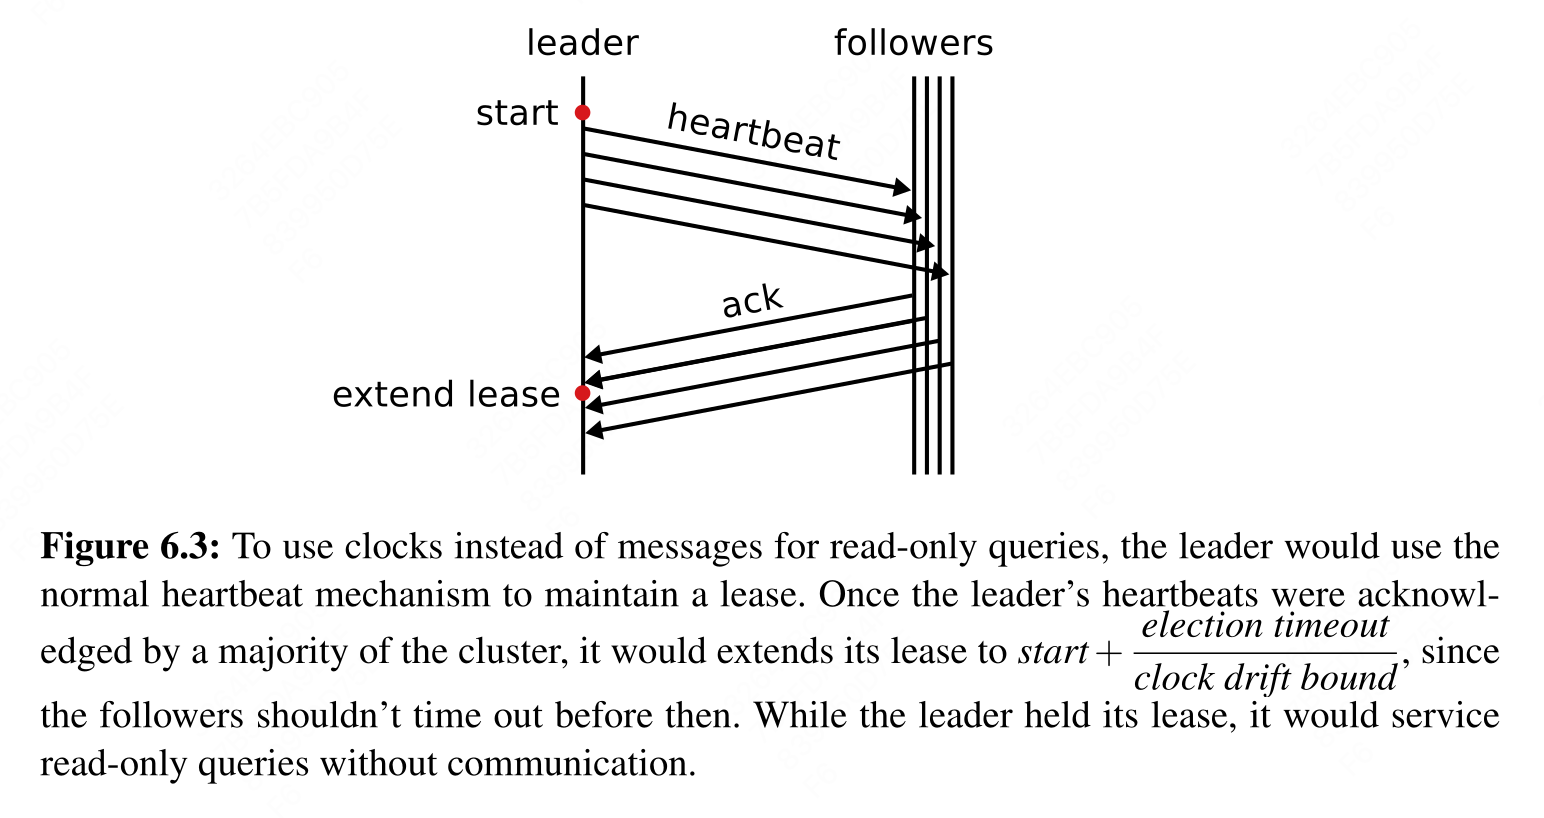
\includegraphics[width=.99\textwidth]{../../images/papers/22.png}
\label{}
\end{center}

The lease approach assumes a bound on clock drift across servers (over a given time period, no
server's clock increases more than this bound times any other). Discovering and maintaining this bound
might present operational challenges.

Fortunately, a simple extension can improve the guarantee provided to clients, so that even under
asynchronous assumptions (even if clocks were to misbehave), each client would see the replicated
state machine progress monotonically (sequential consistency). For example, a client would not
see the state as of log index \(n\), then change to a different server and see only the state as of log
index \(n-1\).
\begin{itemize}
\item To implement this guarantee, servers would include the index corresponding to the state machine
state with each reply to clients. Clients would track the latest index corresponding to results they
had seen, and they would provide this information to servers on each request. If a server received a
request for a client that had seen an index greater than the server’s last applied log index, it
would not service the request (yet).
\end{itemize}
\section{Correctness}
\label{sec:orgdabc022}
\subsection{Formal specification and proof for basic Raft algorithm}
\label{sec:orgaaa39ed}
The specification models an asynchronous system (it has no notion of time) with the following assumptions:
\begin{itemize}
\item Messages may take an arbitrary number of steps (transitions) to arrive at a server. Sending a
message enables a transition to occur (the receipt of the message) but with no particular timeliness.
\item Servers fail by stopping and may later restart from stable storage on disk.
\item The network may reorder, drop, and duplicate messages.
\end{itemize}
\section{Leader election evaluation}
\label{sec:orgf9ff11f}
\subsection{Preventing disruptions when a server rejoins the cluster}
\label{sec:org1d0cb4d}
One downside of Raft’s leader election algorithm is that a server that has been partitioned from the
cluster is likely to cause a disruption when it regains connectivity.

In the Pre-Vote algorithm, a candidate only increments its term if it first learns from a majority of
the cluster that they would be willing to grant the candidate their votes:
\begin{enumerate}
\item if the candidate's log is sufficiently up-to-date
\item voters have not received heartbeats from a valid leader for at least a baseline election timeout
\end{enumerate}
\section{Problem}
\label{sec:org8a2cab6}
\begin{enumerate}
\item \ref{Problem1}: Not quite understand
\item \ref{Problem2}: same roblem
\end{enumerate}
\end{document}
